\documentclass[12pt, a4paper, titlepage, oneside]{book}
\usepackage[utf8]{inputenc}
\usepackage[italian]{babel} %set language = italian
\usepackage{pdfpages} %include function for pdf
\usepackage{mathptmx} %set font type = times 
\textheight24cm\topmargin0mm\headheight0mm\headsep6mm\oddsidemargin20pt\evensidemargin30pt %margin 
\linespread{1.2} %interlinea
\pagestyle{plain}
\usepackage{hyperref}

\usepackage[backend=biber,style=numeric,sorting=none]{biblatex} %bibliography
\usepackage{csquotes}
\addbibresource{bibliography.bib}

\usepackage{titlesec} %style chapter
\titleformat{\chapter}
  {\normalfont\LARGE\bfseries}{\thechapter}{1em}{}
\titlespacing*{\chapter}{0pt}{3.5ex plus 1ex minus .2ex}{2.3ex plus .2ex}

\usepackage{graphicx} %insert image
\graphicspath{ {./images/} }
\usepackage{wrapfig} %for wrap figures
\usepackage{graphicx} %for size figures
\usepackage{subcaption} %for position figures

\usepackage{listings} %for code format
\usepackage{xcolor}
\definecolor{mGreen}{rgb}{0,0.6,0}
\definecolor{mGray}{rgb}{0.5,0.5,0.5}
\definecolor{mPurple}{rgb}{0.58,0,0.82}
\definecolor{backgroundColour}{rgb}{0.95,0.95,0.92}
\lstdefinestyle{CStyle}{
    backgroundcolor=\color{backgroundColour},   
    commentstyle=\color{mGreen},
    keywordstyle=\color{magenta},
    numberstyle=\tiny\color{mGray},
    stringstyle=\color{mPurple},
    basicstyle=\footnotesize,
    breakatwhitespace=false,         
    breaklines=true,                 
    captionpos=b,                    
    keepspaces=true,                 
    numbers=left,                    
    numbersep=5pt,                  
    showspaces=false,                
    showstringspaces=false,
    showtabs=false,                  
    tabsize=2,
    language=C
}
\setlength\parindent{0pt}
%\usepackage{parskip}% http://ctan.org/pkg/parskip
\usepackage[export]{adjustbox}

\begin{document}
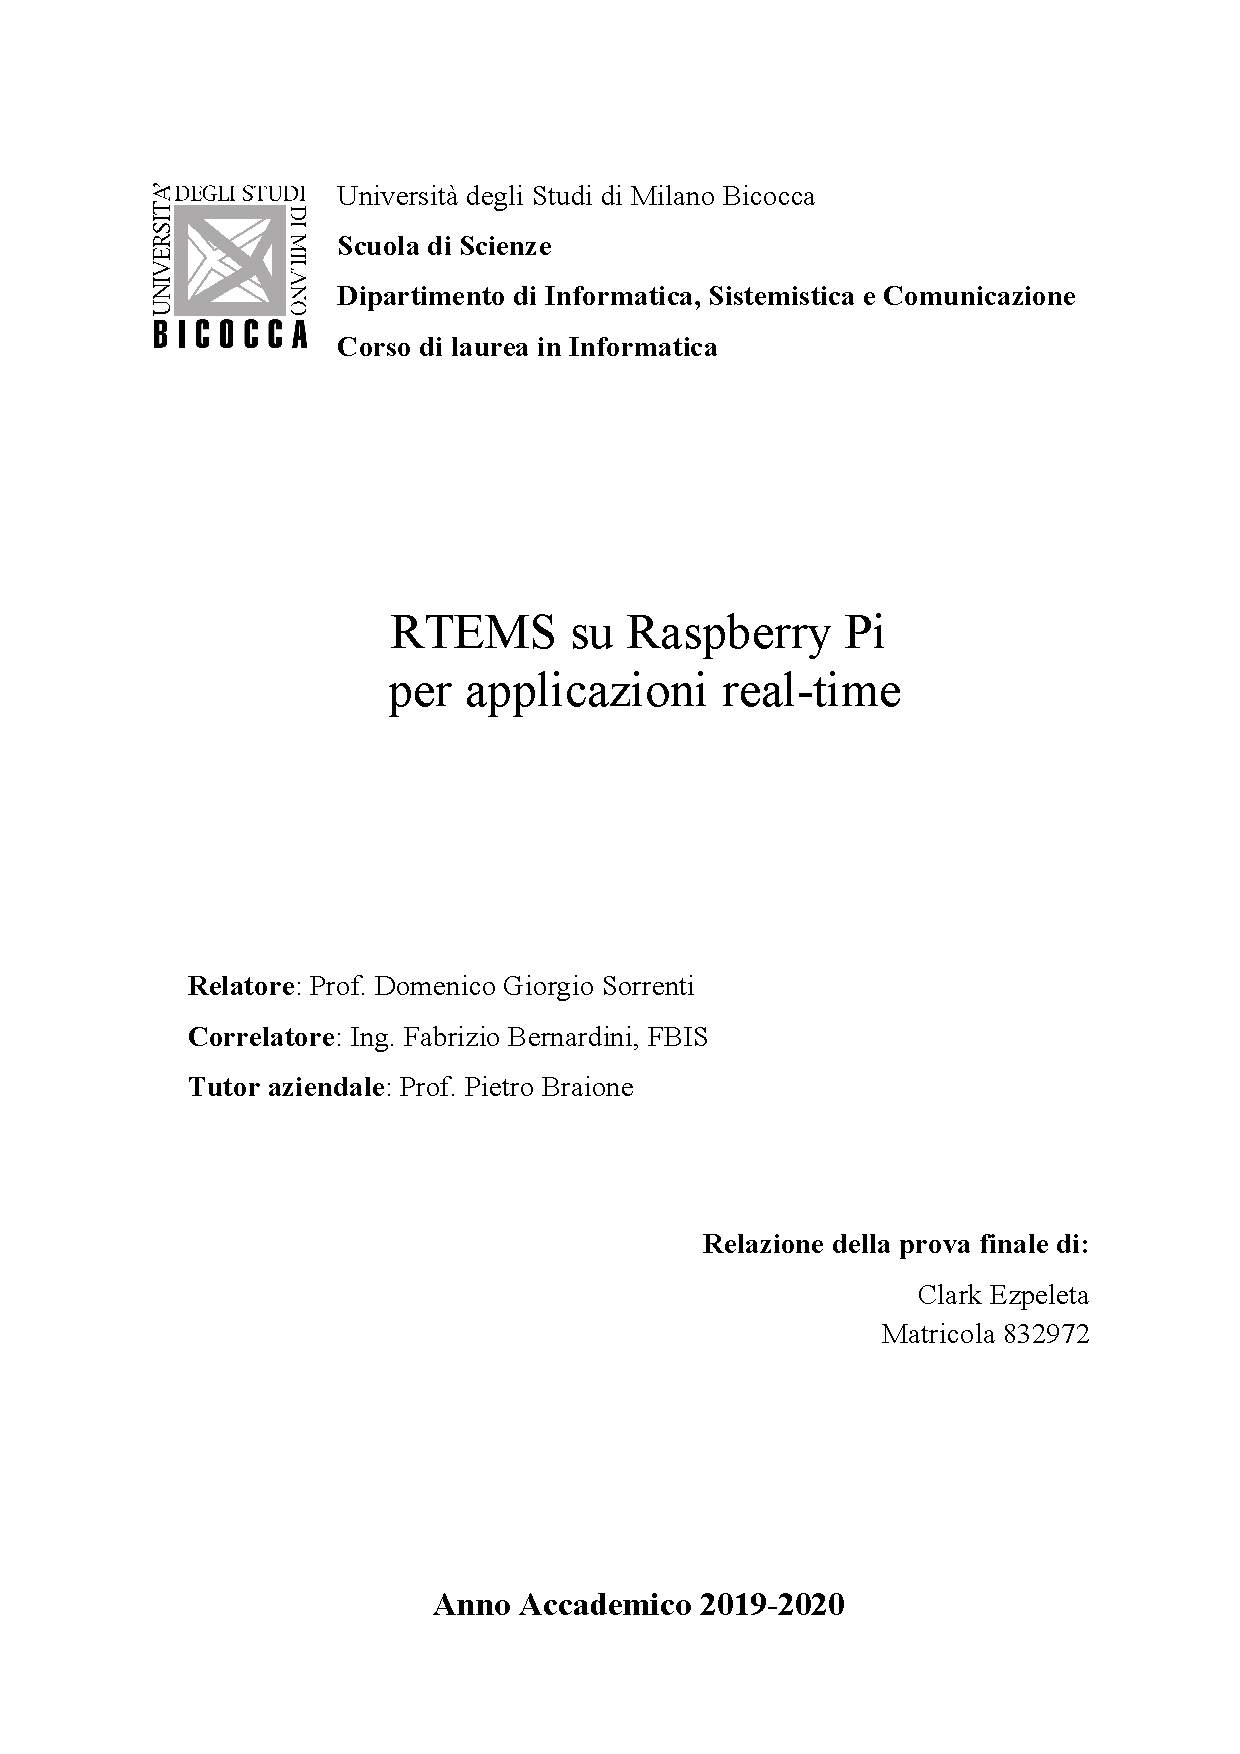
\includepdf[pages={1}]{20210209_Frontespizio_Ezpeleta.pdf}
\tableofcontents
\setcounter{page}{0}
\chapter*{Introduzione}
\setcounter{page}{1}
\addcontentsline{toc}{chapter}{Introduzione} 
%OK
Il lavoro che ho svolto ha due obiettivi principali: il 'porting' di RTEMS su Raspberry Pi e la creazione di applicativi RTEMS per validare il corretto funzionamento delle interfacce GPIO, UART, I2C, SPI  e l'utilizzo degli interrupts tramite le API di RTEMS.\newline
Per  svolgere il 'porting' ho fatto riferimento al RTEMS User Manual\cite{rtemsUM}, per comprendere meglio i concetti di RSB(RTEMS Source Builder) e BSP (board support packages), 
ed ho utilizzato la guida fornita da ing. Basile \cite{giorgio}, di BIS-Italia, che raccoglie tutti i passaggi esposti sul blog di Alan Tech per il 'porting' della versione 4.11.\newline
Purtroppo i passaggi illustrati sul blog non sono totalmente corretti, poiché sono per il 'porting' della versione di RTEMS precedente a quella che ho utilizzato, cioè la 5.1 che è la più recente e stabile.\newline
Il 'porting' può essere definito corretto se alla fine della procedura si riesce a caricare uno degli applicativi di test forniti da RTEMS, su Raspberry Pi senza errori.\newline
Dopo aver effettuato correttamente il 'porting', ho creato una guida in italiano  che raggruppa tutti i passaggi effettuati integrando le correzioni necessarie, ed è stata corretta anche la guida di ing. Basile \cite{giorgio5}.
Dopo aver impostato l'ambiente di lavoro ho iniziato a creare gli applicativi RTEMS da eseguire sulla Raspberry Pi.\newline
Per  creare gli applicativi RTEMS ho dovuto  familiarizzare con il linguaggio C, leggere l'RTEMS Classic API Guide \cite{rtemsCAG} ed analizzare i codici sorgente di esempio trovati nel git repository di asuol\cite{asuol} per  comprendere l'utilizzo delle API. \newline
Tutto il lavoro è stato eseguito in modalità "smart-working", per questo motivo mi è stata messa a disposizione da BIS-Italia la scheda Raspberry Pi 3B+ per  effettuare l'attività. Inoltre Microchip Technologies ha gentilmente offerto dei componenti aggiuntivi utili per gli applicativi RTEMS di test dell'interfaccia I2C e SPI.\newline
Oltre all'attività software ho dovuto eseguire una piccola attività hardware, cioè creare dei circuiti saldando i vari componenti e utilizzando la breadboard in modo da collegarli alla Raspberry Pi, per fare ciò ho seguito gli schemi elettrici che mi ha inviato ing. Bernardini e ho letto i datasheet dei componenti dell'interfaccia I2C \cite{microchipMCP3425} \cite{microchipADC} e  SPI \cite{microchipMCP4822} \cite{microchipMSOP10-8} in modo da comprendere il loro funzionamento e  creare i driver.
\newpage
Premesso tutto ciò ho suddiviso la mia relazione nei seguenti capitoli:
\begin{itemize}
    \item \textbf{Capitolo 1} - in questo capitolo vengono descritte le principali tecnologie utilizzate durante il mio lavoro. Innanzitutto viene descritto RTEMS che è il sistema operativo su cui si basa tutta l'attività, dopodiché viene  descritta la Raspberry Pi su cui verranno eseguiti gli applicativi RTEMS, ed infine viene descritto Eclipse che è l'IDE utilizzato per creare gli applicativi.
    \item \textbf{Capitolo 2} - in questo capitolo viene fatta una sintesi di tutta l'attività di 'porting', e la definizione della toolchain per realizzare gli applicativi RTEMS. Vengono esposte tutte le problematiche riscontrate e le loro soluzioni.
    Per informazioni più dettagliate riguardo il procedimento si rimanda alla guida in appendice.
    \item \textbf{Capitolo 3} - in questo capitolo vengono descritti le API che RTEMS ha a disposizione, la loro struttura e in che modo sono stati validati e per quali motivi si è scelto di testarli.
    \item \textbf{Capitolo 4} - in questo capitolo viene descritta l'attività software che si basa sulla creazione degli applicativi RTEMS per testare il corretto funzionamento delle API di RTEMS. Viene esposto anche una descrizione dei componenti aggiuntivi offerti da Microchip di cui sono stati creati i driver per utilizzarli con RTEMS.
    \item \textbf{Capitolo 5} - in questo capitolo viene descritto ciò che si è raggiunto e la possibile estensione del mio lavoro.
\end{itemize} 
Questo lavoro è stato sviluppato in collaborazione con la sezione italiana della British Interplanetary Society, che utilizzerà i risultati in alcuni progetti futuri.

\begin{figure}[b]
    \centering
    
\includegraphics[scale = 0.15, left]{images/BIS-Italia_logo_new_big.png}
\end{figure}
\chapter{Tecnologie}
\section{RTEMS}
\begin{figure}[h]
    \centering
    
\includegraphics[scale = 2]{rtemslogo.png}
\end{figure}
RTEMS sta per\textbf{ Real-Time Executive MultiProcessor System} ed è un sistema operativo real-time (RTOS) general purpose open source (licenza GPL 2.0 modificata) progettato e gestito da OAR Corporation. Il suo sviluppo iniziò nella fine degli anni 80 utilizzando i linguaggi Ada e C, e venne usato inizialmente per scopi militari, invece le prime versioni utilizzabili sono state rese open-souce su server ftp nel 1994.\newline
Attualmente viene utilizzato in molti settori tra cui quello aerospaziale, infatti è stato utilizzato in alcune missioni spaziali sia a livello di on-board computer che come computer embedded in altre attività di volo.\newline
%ad esempio sul MRO (Mars Reconnaissance Orbiter) è in esecuzione un applicativo RTEMS che controlla l' Electra UHT Transceiver (EUT) che serve per la comunicazione tra Marte e la Terra . \newline
RTEMS è  stato\textbf{ validato dall'ESA}, European Space Agency, ciò vuol dire che sono stati scritti dei programmi che riproducono gli scenari critici (ad esempio la gestione di molti dispositivi oppure la gestione e l'esecuzione concorrente dei task), e sono stati eseguiti sul sistema operativo per poter verificare il suo corretto funzionamento in quei casi. La validazione viene tutt'ora aggiornata poiché è un sistema operativo che è in continua evoluzione e avrà più funzionalità con il passare del tempo.\newline
\textbf{RTEMS} non è un sistema operativo a sé stante, usato per caricare altri programmi, ma \textbf{è un executive} che viene compilato con l'applicazione in un unico codice monolitico da eseguire.\newline
RTEMS è usto per applicazioni categoria 13 (mission critical) in molti veicoli spaziali della NASA e dell'ESA
\newpage

RTEMS può anche essere visto come un insieme di direttive raggruppate in una serie di \textbf{manager}, che si occupano di varie funzionalità tra cui il controllo e la sincronizzazione dei task e processori, la gestione della memoria e la mutua esclusione. Invece la gestione dello scheduling, dispatching e object management sono forniti dal executive core.
\begin{figure} [h]
    \centering
    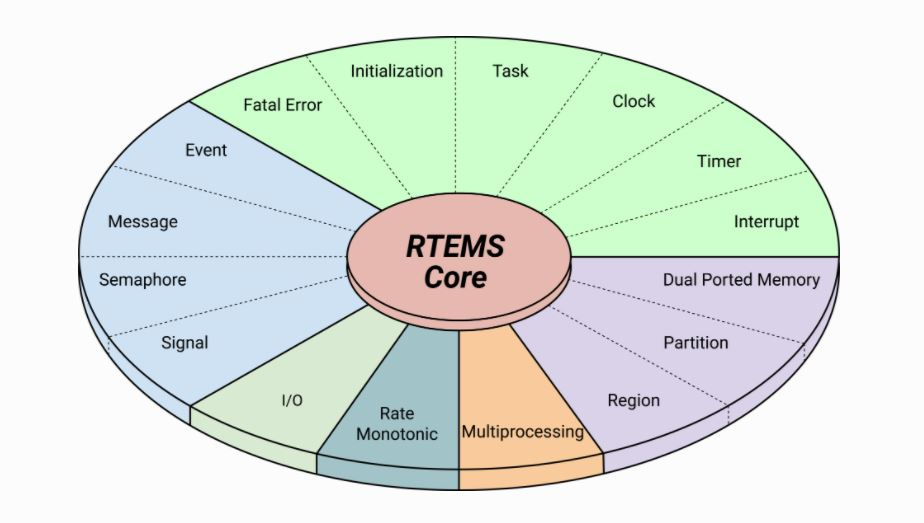
\includegraphics[scale = 0.75]{rtems_internal_architecture.JPG}
    \caption{Architettura RTEMS}
    \label{fig:my_label1}
\end{figure}
Utilizzando i managers di RTEMS lo sviluppatore può concentrarsi al solo sviluppo del applicativo e ciò riduce notevolmente il tempo di sviluppo.\newline
La figura successiva mostra la logica di utilizzo di RTEMS.
\begin{figure}[h]
    \centering
    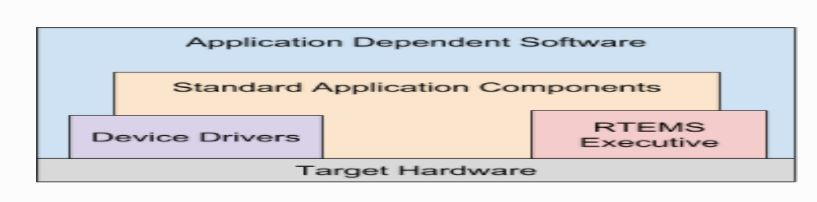
\includegraphics[scale = 0.75]{application_architecture.JPG}
    \caption{Struttura applicativo RTEMS}
    \label{fig:my_label2}
\end{figure}
Come si può notare RTEMS Executive è un intermediario tra il codice dell'applicativo e il target hardware, invece le dipendenze hardware con altri device sono localizzati nel livello "device drivers".
Il RTEMS I/O manager incorpora queste dipendenze hardware nel sistema mentre allo stesso momento fornisce all'application code l'accesso ad esse.
Queste dipendenze hardware sono isolate in specifiche \textbf{BSP}, Board Support Packages, per questo motivo il 'porting' di un applicativo RTMES su altri processori è semplice poiché basterebbe selezionare il BSP del microprocessore su cui si vuol eseguire l'applicativo e compilare con le sue librerie.\newline
In questo modo durante lo sviluppo di un applicativo real-time si ha la totale indipendenza dall'architettura dei microprocessori. \newline
È disponibile il 'porting' di RTEMS su molte architetture CPU tra cui\textbf{ ARM}, MIPS, LEON,ERC32 e i PowerPC; durante il questo lavoro viene trattato il 'porting' su architettura ARM utilizzando una Raspberry Pi 3B+.
\section{Raspberry Pi}
\begin{figure}[h]
    \centering
    
\includegraphics[scale = 0.70]{raspberrypiLogo.png}
\end{figure}
Raspberry Pi è una serie di computer a scheda singola sviluppata da Raspberry Pi Foundation in collaborazione con la Broadcom, in Inghilterra.\newline
Originariamente è stato usato per insegnare le basi dell'informatica nelle scuole e nei paesi in via di sviluppo, ma attualmente grazie al suo basso prezzo viene utilizzato anche nel settore della robotica, domotica e in molti altri.
Al momento sono state rilasciate quattro generazioni di Raspberry Pi, e tutti i modelli hanno un Broadcom SoC (System on Chip) con processore ARM integrato e on-chip GPU (Graphics Processing Unit).\newline
In questo lavoro viene usata la \textbf{Raspberry Pi 3B+} che utilizza il Broadcom BCM2837B0 SoC \cite{bcm2837} con processore Cortex-A53 (ARMv8) 64-bit 1.4Ghz.
\newpage
\begin{figure} [h]
    \centering
    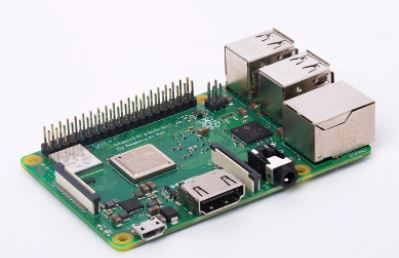
\includegraphics[scale = 1.25]{RPi3B.JPG}
    \caption{Scheda Raspberry Pi 3B+}
    \label{fig:RPI3B_laver}
\end{figure}
Tra le specifiche tecniche quelle che ci interessano maggiormente sono:
\begin{itemize}
    \item SDRAM LPDDR2 da 1GB.
    \item supporto per la micro SD.
    \item accesso a 40 GPIO.
\end{itemize}

La scheda micro SD deve essere configurata nel seguente modo:
\newline
\begin{enumerate}
    \item copiare il firmware di Raspberry Pi compatibile con RTEMS nella memoria SD.
    \item cancellare i file 'kernel*.img'. 
    \item compilare i sorgenti di un applicativo RTEMS in modo da ottenere il file con estensione'.img' 
    \item copiare l'eseguibile RTEMS nella memoria SD.
    \item \parbox[t]{\linewidth}{impostare l'eseguibile RTEMS come kernel della scheda Raspberry Pi, modificando il file 'config.txt' aggiungendo il comando "kernel=nome\_eseguibile.img"}
\end{enumerate}

Ulteriori dettagli sono forniti nella guida validata come parte di questo lavoro e disponibile in allegato a questa relazione.
Questi passaggi sono necessari poiché il 'bootloader' di Raspberry Pi 3B+ è preimpostato in modo che, quando viene accesa la scheda, cerca un file denominato "kernel7.img" per caricare il sistema operativo. In questo caso non viene caricato un sistema operativo ma un eseguibile basato su RTEMS, che quando avviato prende il totale controllo della scheda.

\newpage
La figura successiva mostra tutti i pin GPIO che Raspberry Pi 3B+ ha a disposizione:
\begin{figure}[h]
    \centering
    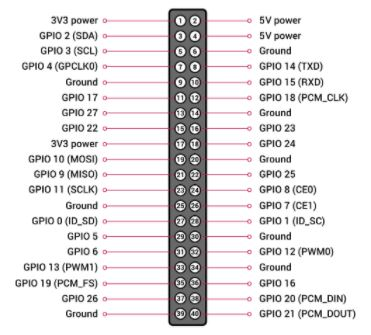
\includegraphics[scale = 1.40]{RPi3B_GPIO.JPG}
    \caption{Raspberry Pi 3B+ GPIO}
    \label{fig:RPi3B_GPIO}
\end{figure}

Nella scheda i livelli logici sono così definiti : alto se la tensione è pari a 3V3 e ciò corrisponde al valore binario 1, basso se la tensione è pari a 0V e ciò corrisponde al valore binario 0.\newline 
I pin configurabili come input sono 3V3 'tolerant', quindi ricevono in input una tensione che va da 0v a 3V3, ed ogni pin ha una resistenza di pull-down o pull-up che è possibile impostare da software.
I pin configurabili come output possono dare una tensione da 0V a 3V3.\newline
Infine alcuni pin possono essere utilizzati anche per gestire altre interfacce come l'I2C, UART, SPI.\newline
I files per il 'porting' di RTEMS offrono i 'drivers' per accedere a queste interfacce in un BSP (Board Support Package) che è stato verificato in parte durante questo lavoro.
\newpage
\section{Eclipse}
Eclipse è un IDE open source rilasciato con licenza EPL (Eclipse Public License) creato da IBM usato principalmente per la programmazione in Java ma grazie a vari plugin può essere usato per altri linguaggi di programmazione come C, C++, COBOL, Python e molti altri. \newline
L'ambiente di sviluppo Eclipse include l'Eclipse Java development tools per Java, e l'Eclipse CDT per C/C++. \newline
Per utilizzare "RTEMS gcc cross compiler" su Eclipse C, bisogna installare il plugin di RTEMS e settare le variabili di ambiente.
\begin{figure} [h]
    \centering
    \includegraphics[height = 135mm, width = 160mm ]{eclipse-i2c.png}
    \caption{Schermata Eclipse del programma I2C }
    \label{fig:eclips-i2c}
\end{figure}
\chapter{Porting di RTEMS su Raspberry Pi }
%OK
L'attività di 'porting' è la prima fase del lavoro e consiste in:
\begin{enumerate}
    \item Installazione dalla tool-suite sul computer host, dove vengono creati gli applicativi RTEMS.
    \item Verifica del corretto funzionamento della tool-suite, eseguendo i programmi di test su Raspberry Pi
    \item Configurazione del IDE Eclipse C, per la creazione di eseguibili RTEMS
    \item Compilazione ed esecuzione dei programmi sia da terminale, e sia da Eclipse C
\end{enumerate}
Per svolgere tutta la procedura bisogna essere muniti di un computer con sistema operativo Ubuntu, una scheda Raspberry Pi 3B+, una micro SD, e convertitore TTL USB.\newline
RTEMS in sé è complesso per questo il team di RTEMS ci fornisce "l'ecosistema di RTEMS" che è una collezione di strumenti, packages, codici sorgente e documentazione, utile per definire come sviluppare, mantenere e usare RTEMS.\newline
Durante il 'porting' vengono utilizzati due importanti strumenti che fanno parte dell'ecosistema RTEMS, e sono :
\begin{itemize}
    \item\parbox[t]{\linewidth}{\textbf{RTEMS RSB}: il RTEMS Source Builder è tool molto utile per compilare e fare la 'build' dei moduli di RTEMS e delle BSP}
    \item\parbox[t]{\linewidth}{\textbf{BSP raspberrypi}: la Build Support Package è il codice di supporto, che contiene le librerie di RTEMS per una specifica scheda (ad esempio il BSP raspberrypi viene usata per la Raspberry Pi 3B+)}
\end{itemize}
\textbf{L'installazione della tool-suite e BSP }viene fatta tutta tramite comandi su terminale, non esiste un eseguibile .exe, ma viene usato il RTEMS RSB.\newline
Ci sono due requisiti necessari da rispettare e sono, avere installato Git per scaricare il codice sorgente di RTEMS, ed essere in grado di compilare i programmi C/C++ e Python poiché molti moduli della tool-suite sono scritti con questi linguaggi.\newline
La versione di cui bisogna effettuare il porting è la \textbf{5.1} che è la più recente e stabile, anche se ciò ha dato problemi durante l'installazione perché la guida a cui si faceva riferimento era per la versione precedente 4.1 rilasciata nel 2015, e veniva clonato il ramo main dove attualmente è presente una versione ancora in sviluppo.\newline
Grazie all'aiuto dell'ing. Basile, siamo riusciti a capire che il problema stesse nel comando git che clonava la versione in sviluppo sul 'branch' master. Quindi dopo aver 'clonato' la versione corretta viene installata la "RTEMS tool-suite" e il BSP di Raspberry Pi \newline
il BSP "raspberrypi" dà a disposizione, oltre alle librerie di supporto per l'utilizzo della scheda, dei programmi .exe da compilare ed eseguire sulla scheda, in modo da verificare che l'installazione sia stata effettuata con successo.\newline
L'\textbf{esecuzione degli applicativi di esempio} sulla scheda non dava i risultati previsti, poiché l'ultima versione del firmware di Raspberry Pi copiato sulla scheda SD non è compatibile con RTEMS, e quindi si è dovuto ricercare il firmware compatibile. Dopo aver copiato il firmware corretto della Raspberry Pi sulla scheda SD, e verificato il funzionamento della scheda con gli applicativi d'esempio, si passa alla creazione degli applicativi RTEMS.\newline
Per creare i file sorgenti di un applicativo RTEMS si può usare un semplice editor di testo per poi compilarli con il 'gcc cross compiler' di RTEMS tramite terminale, oppure utilizzare l'IDE Eclipse C/C++ per semplificare il processo.\newline
L'\textbf{IDE Eclipse deve essere configurato} installando il plugin "RTEMS CDT support" ed impostando le variabili d'ambiente, in modo da "puntare" al gcc cross compiler di RTEMS e il BSP corretto.\newline
Per verificare che tutto l'ambiente sia stato impostato correttamente, viene \textbf{creato un semplice programma "hello world"}, che manda tramite UART il messaggio su terminale. L'applicativo inizialmente non mandava il log come ci si aspettava, ed il problema risiedeva nella configurazione del sistema definito nell'applicativo, che inizializzava il driver della console errato, e il driver del clock, che in questo caso era inutile.\newline
La compilazione del programma "hello world", che può essere effettuata sia da terminale che da Eclipse, non ha dato nessun problema di compilazione. A questo punto viene caricato sulla Raspberry Pi e si ha la conferma della correttezza del applicativo visualizzando sul terminale il log "Hello World" come previsto.\newline
\textbf{A questo punto del lavoro è stata creata una guida }che espone tutti i passaggi corretti, cosicché qualunque utente voglia approcciarsi ad RTEMS su Raspberry Pi per la prima volta riesca a fare il porting senza dover cercare tra le tante fonti sparse su internet.\newline
\textbf{Per informazioni più dettagliate riguardo i passaggi del 'porting' è disponibile, in appendice, la guida prodotta durante il tirocinio}

\chapter{Integrazione hardware e software}
%Qui ci va una descrizione delle varie interfacce disponibili in termini di drivers SW e come le abbiamo provate.
%TO CHECK
Effettuato il 'porting' si può procedere con l'attività software, cioè la creazione di RTEMS executive per validare il funzionamento delle RTEMS Classic API che sono le API per l'utilizzo delle interfacce. \newline
\begin{figure} [h]
\centering
    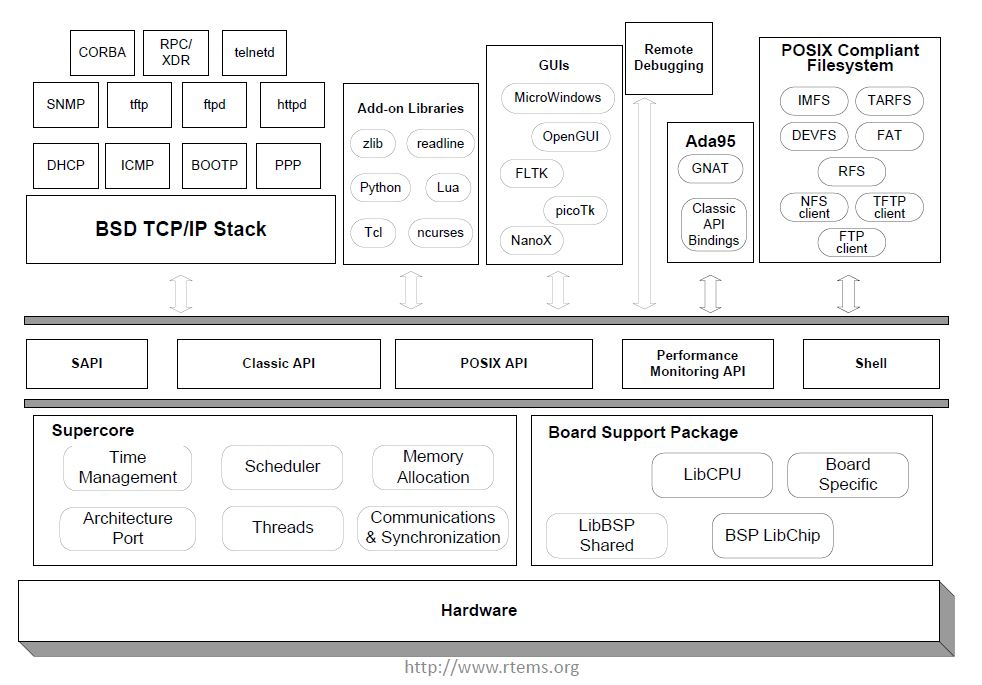
\includegraphics[scale = 0.75] {RTEMS_architecture.JPG}
    \caption{Architettura dettagliata sistema RTEMS}
    \label{fig:my_label3}
\end{figure}
Le interfacce che ci interessano validare sono:UART, GPIO, I2C, SPI.\newline
In futuro sarà possibile anche aggiungere un'interfaccia per il bus CAN utilizzando componenti che usano l'interfaccia SPI.
il BSP dà a disposizione API e drivers per utilizzare le interfacce che ci interessano.\newline
\newpage
La figura successiva mostra la struttura ed alcuni driver, file di configurazione e librerie presenti nel BSP, utili per l'attività sperimentale:
\begin{figure} [h]
\centering
    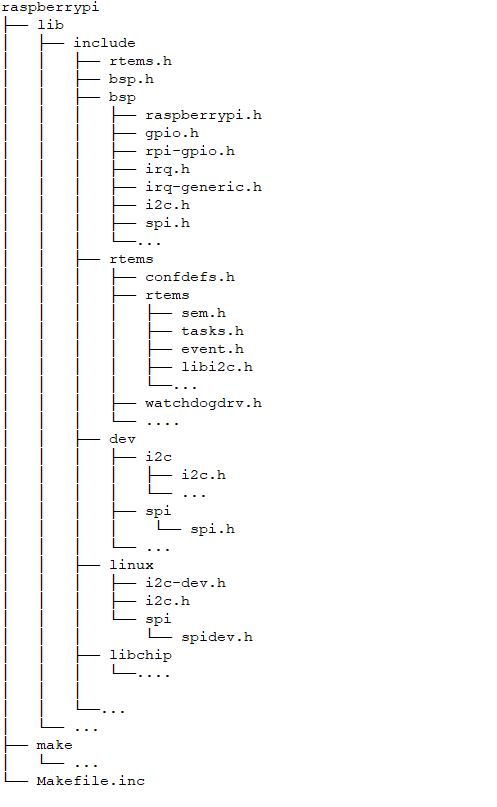
\includegraphics[scale = 1.0] {BSP_DIR_TREE.JPG}
    \caption{Struttura file BSP}
    \label{fig:Struttura cartelle BSP}
\end{figure}
\newpage
\begin{itemize}
    \item\parbox[t]{\linewidth}{ rtems.h : serve ad interfacciarsi ed includere tutte le RTEMS Classic API}
    \item\parbox[t]{\linewidth}{bsp.h : definisce le macro per la Rasperry Pi*}
    \item\parbox[t]{\linewidth}{bsp/raspberrypi.h : definisce i registri della Raspberry Pi}
    \item\parbox[t]{\linewidth}{bsp/gpio.h : definisce le API per la gestione dei GPIO}
    \item\parbox[t]{\linewidth}{bsp/rpi-gpio.h : definisce le API per i GPIO specifiche per la Raspberry Pi}
    \item\parbox[t]{\linewidth}{bsp/irq.h : definisce le macro per utilizzare gli interrupt}
    \item\parbox[t]{\linewidth}{bsp/irq\_generic.h : definisce le API per la gestione degli interrupts}
    \item\parbox[t]{\linewidth}{bsp/i2c.h : definisce le API per I2C specifiche per la Raspberry Pi}
    \item\parbox[t]{\linewidth}{bsp/spi.h : definisce le API per SPI specifiche per la Raspberry Pi}
    \item\parbox[t]{\linewidth}{rtems/confdefs.h : serve a configurare il sistema su cui gira l'applicativo}
    \item\parbox[t]{\linewidth}{rtems/rtems/sem.h : definisce le API per gestire i semafori}
    \item\parbox[t]{\linewidth}{rtems/rtems/tasks.h : definisce le API per la gestione dei task}
    \item\parbox[t]{\linewidth}{rtems/rtems/event.h : definisce le API per la gestione degli eventi}
    \item\parbox[t]{\linewidth}{ dev/i2c/i2c.h : definisce l'I2C driver framework ed è compatibile con la Linux I2C user-space API}
    \item\parbox[t]{\linewidth}{ dev/spi/spi.h :  definisce il SPI driver framework ed è compatibile con la Linux SPI user-space API}
\end{itemize}

L'elenco sopra rappresenta è solo una\textbf{ piccola estrazione di cio che il BSP contiene}.\newline
Si fa notare che il BSP per RaspberryPi è un prodotto "open-source" messo a disposizione su Internet senza partiolari garanzie di affidabilità e di completezza.\newline
Questo ha creato dei problemi che hanno rallentato molto il lavoro.\newline
\chapter{Attività sperimentale}
%OK
\section{Obiettivi}
L'attività sperimentale consiste nella creazione di applicativi RTEMS per validare le API di RTEMS. Un API può essere considerata valida se l'applicativo, eseguito sulla scheda, dia il risultato prestabilito e nell'arco temporale definito.\newline
\section{Test set-up}
Ogni programma di test creato implica un circuito elettrico differente costruito con jumper, breadboard, resistenze, condensatori, pulsanti, LED e schede aggiuntive fornite dalla Microchip su cui vengono saldati cavetti e componenti per poterli utilizzare e collegare alla Raspberry Pi.\newline
I componenti aggiuntivi sono :
\begin{itemize}
    \item\parbox[t]{\linewidth}{ \textbf{MCP3425 SOT23-6 Evaluation Board}  \cite{microchipMCP3425}: un evaluation board, con un ADC (Analog Digital Converter) MCP3425, controllato tramite protocollo I2C}
    \item\parbox[t]{\linewidth}{\textbf{MSOP-10 and MSOP-8 Evaluation Board} \cite{microchipMSOP10-8}: un evaluation board generica che serve per il collegamento del componente MCP4822 alla Raspberry Pi}
    \item\parbox[t]{\linewidth}{\textbf{ MCP4822} \cite{microchipMCP4822}: un DAC (Digital Analog Converter) controllato tramite protocollo SPI, montato sulla evaluation board sopracitata.}
\end{itemize}
\newpage
Il componente \textbf{MCP3425} è un ADC, 'Analog Digital Converter', da 16 bit a canale singolo e vengono passati come input due tensioni ai pin $V_{IN}^+ $ e $ V_{IN}^-$ e viene restituito come output una tensione pari a $V_{IN}^+ - V_{IN}^- \times PGA$ ('Programmable Gain Amplifier') sul pin SDA (linea dati).\newline 
\begin{figure}[h]
\begin{subfigure}{0.5\textwidth}
    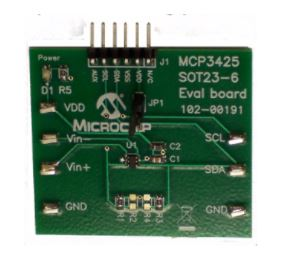
\includegraphics[width=0.9\linewidth, height=7cm]{MCP3425.JPG}
    \caption{MCP3425}
    \label{fig:MCP3425}
\end{subfigure}
\begin{subfigure}{0.5\textwidth}
    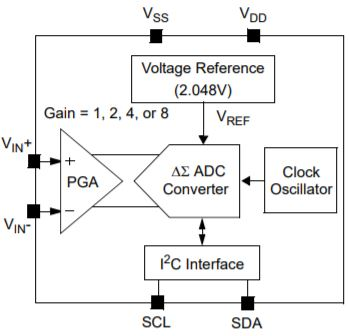
\includegraphics[width=0.9\linewidth, height=7cm]{images/MCP3425_block_diagram.JPG}
    \caption{schema a blocchi di MCP3425}
    \label{fig:MCP3425 block diagram}
\end{subfigure}
\end{figure}
Il componente ha la seguente configurazione predefinita:
\begin{itemize}
    \item Programmable Gain Amplifier(PGA) = 1
    \item Continuos Conversion
    \item Programmable Data Rate = 12 bit
\end{itemize}
Durante il lavoro viene utilizzata questa configurazione, ma nel caso si volesse cambiare la configurazione del componente, si può eseguire una scrittura di due byte dove il primo byte rappresenta l'indirizzo di periferica e il bit R/W (nel nostro caso è 11010000, dove R/W = 0 significa che stiamo eseguendo una scrittura) invece il secondo byte contiene i bit di configurazione\newline
\begin{figure}[h]
    \centering
    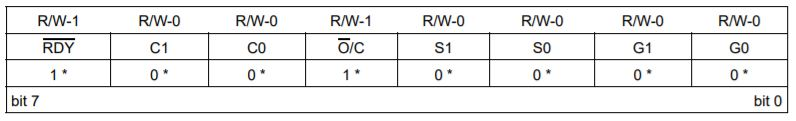
\includegraphics[scale = 0.9]{images/MCP3425_Configuration_register.JPG}
    \caption{Registro di configurazione MCP3425 con la configurazione preimpostata}
    \label{fig:CONFIG_REG_MCP3425}
\end{figure}
\newpage
\begin{figure}[h]
    \centering
    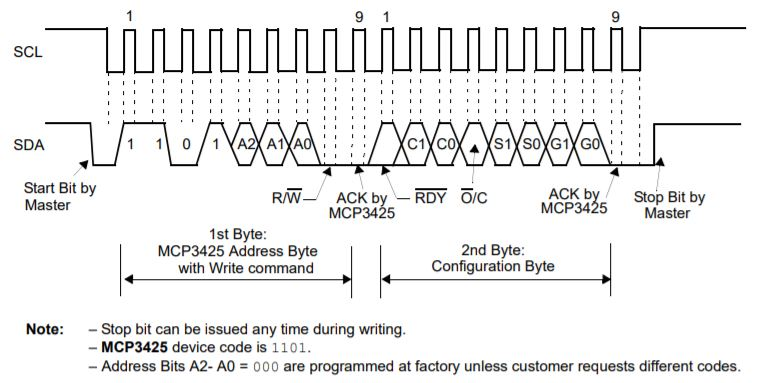
\includegraphics[scale = 0.95]{wrtie_configuration_MCP3425.JPG}
    \caption{Diagramma temporale scrittura su MCP3425}
    \label{fig:MCP3425_write_conf}
\end{figure}
Su questo componente ci interessa effettuare la lettura della tensione in uscita che è rappresentata da due byte. Per eseguire la lettura bisogna seguire questi passaggi:
\begin{enumerate}
    \item Mandare sul bus I2C l'indirizzo di periferica con R/W pari a 1.
    \item Lettura dei due byte.
    \item Eseguire la conversione dei byte per avere il valore effettivo della tensione.
\end{enumerate}

Dato che viene utilizzata la configurazione preimpostata, in cui viene effettuata una conversione di 12 bit del dato, si ha che nei due byte che riceviamo il dodicesimo bit rappresenta il segno e viene ripetuto fino al sedicesimo bit, quindi non bisogna considerare gli ultimi quattro bit.
Discorso analogo per la conversione in 14 bit e 16 bit.

\begin{figure}[h]
    \centering
    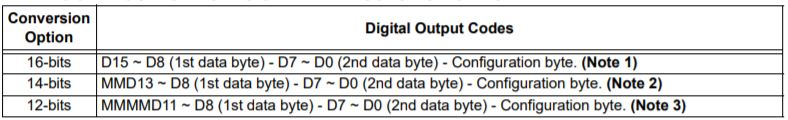
\includegraphics[scale = 0.95]{images/MCP3425_OUTPUT.JPG}
    \caption{Output MCP3425}
    \label{fig:MCP3425graph}
\end{figure}

\newpage
Il componente \textbf{MCP4822} è un DAC, 'Digital Analog Converter', da 12 bit a due canali e come input viene passato da programma 2 byte in cui viene rappresentato il dato da convertire e come output una tensione pari a $V_{OUT} = \frac{V_{ref} \times D_n}{2^n} \times G$ dove:
\begin{itemize}
    \item $V_{ref}$ = 2.048V
    \item $D_n$ = sono i bit che passo in input
    \item $n$ = è il numero dei bit, cioè 12
    \item $G$ = è il guadagno
\end{itemize}

%\begin{figure}[h]
%\begin{subfigure}{0.5\textwidth}
%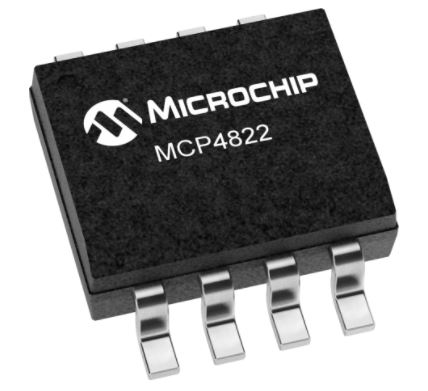
\includegraphics[width=0.8\linewidth, height=3cm]{images/MCP4822.JPG} 
%\caption{MCP4822}
%\label{fig:MCP4822}
%\end{subfigure}
%\begin{subfigure}{0.5\textwidth}
%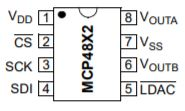
\includegraphics[width=0.7\linewidth, height=3cm]{images/MCP4822_pin.JPG}
%\caption{MCP4822 pin}
%\label{fig:MCP4822 pin}
%\end{subfigure}
%\end{figure}

\begin{figure} [h]
    \centering
    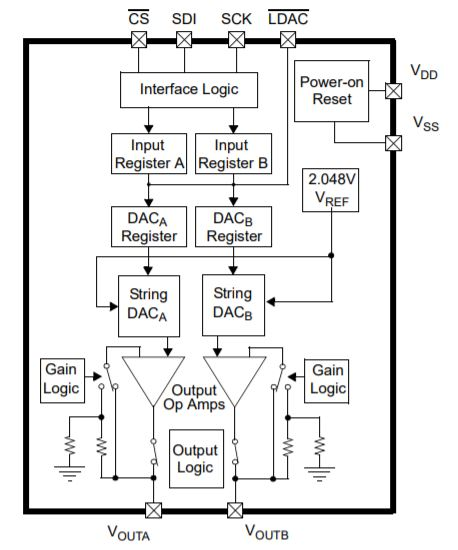
\includegraphics[scale = 1]{images/MCP4822_block_diagram.JPG}
    \caption{Schema a blocchi di MCP4822}
    \label{fig: MCP4822 BLOCK DIAGRAM}
\end{figure}

Il componente ha due canali e la comunicazione è unidirezionale, cioè può essere eseguita solo la scrittura.\newline
Durante il lavoro verrà utilizzato solo un canale (canale A).\newline
\newpage
La scrittura viene effettuata mandando due byte di cui il primo è formato dai 4 bit di configurazione e gli ultimi 4 data bit, e il secondo è formato dai restanti data bit.\newline
\begin{figure}[h]
    \centering
    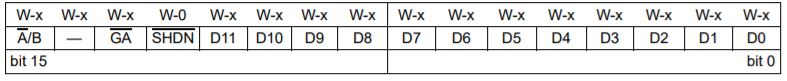
\includegraphics[scale = 0.95]{images/MCP4822_config_register.JPG}
    \caption{Registro di configurazione del MCP4822}
    \label{fig:MCP4822_CONF_REGISTER}
\end{figure}
Il ciclo di scrittura è definito dal seguente diagramma temporale:
\begin{figure}[h]
    \centering
    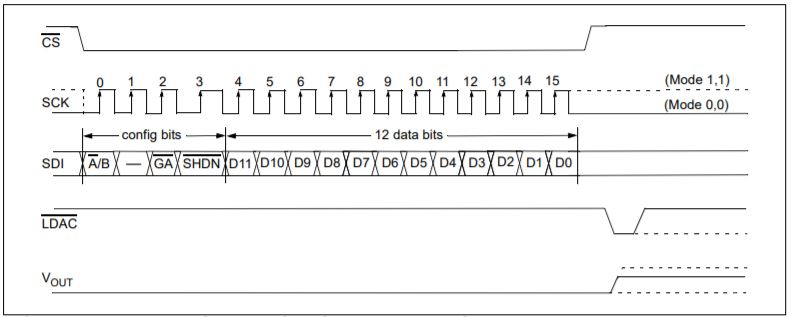
\includegraphics[scale = 0.95]{images/MCP4822_write_time_diagram.JPG}
    \caption{Diagramma temporale scrittura su MCP4822}
    \label{fig:MCP4822 TIME DIAGRAM}
\end{figure}

Effettuata la scrittura del dato sul 'Input Register A' questo viene poi convertito, e il risultato 
\newpage
\section{Test application software}
La struttura principale che tutti i programmi seguono è la seguente:
\begin{itemize}
    \item \textbf{init.c}: è il file sorgente contenente la funzione Init che è il punto di partenza dell'eseguibile. Viene utilizzato come se fosse il metodo main in Java.
    \item \textbf{init.h}: è un file header che contiene tutte le direttive RTEMS per configurare il sistema
    \item \textbf{task\_helper.c}: è il file sorgente contenente la definizione dei task, le funzioni per la manipolazione delle variabili globali, le funzioni aggiuntive 
    \item \textbf{task\_helper.h}: è un file header che contiene tutte le dichiarazioni delle funzioni definite in task\_helper.c che si vogliono usare in init.c, ad esempio la definizione dei task.
\end{itemize}
La configurazione del sistema viene definita tramite le direttive RTEMS, e si può definire una configurazione di base :
\begin{lstlisting}[style = CStyle]
#define CONFIGURE_APPLICATION_DOES_NOT_NEED_CLOCK_DRIVER
#define CONFIGURE_APPLICATION_NEEDS_SIMPLE_CONSOLE_DRIVER
#define CONFIGURE_UNLIMITED_OBJECTS
#define CONFIGURE_UNIFIED_WORK_AREAS
#define CONFIGURE_RTEMS_INIT_TASKS_TABLE
#define CONFIGURE_INIT
#include <rtems/confdefs.h>
\end{lstlisting}
\begin{itemize}
    \item \parbox[t]{\linewidth}{CONFIGURE\_APPLICATION\_DOES\_NOT\_NEED\_CLOCK\_DRIVER: è necessario definirlo quando non si vuole utilizzare il driver del clock e del timer. Nel caso si voglia inizializzare il driver del clock bisogna utilizzare la direttiva CONFIGURE\_APPLICATION\_NEEDS\_CLOCK\_DRIVER, e impostare i microsecondi per tick con la direttiva CONFIGURE\_MICROSECONDS\_PER\_TICK, altrimenti di vengono impostati 10000 microsecondi per tick.}
    \item \parbox[t]{\linewidth}{CONFIGURE\_APPLICATION\_NEEDS\_SIMPLE\_CONSOLE\_DRIVER: imposta il "Simple Console Driver", in questo modo possiamo utilizzare la funzione "printf()" per la visualizzazione dei log.}
    \item \parbox[t]{\linewidth}{CONFIGURE\_UNLIMITED\_OBJECTS: con questa direttiva non si ha limiti di oggetti rtems, e non si ha il bisogno di gestire la RAM. Ovviamene questa direttiva non deve essere usata per applicativi da mandare in produzione, ma può essere usata durante la fase di test}
    \item \parbox[t]{\linewidth}{CONFIGURE\_UNIFIED\_WORK\_AREAS: da utilizzare quando la direttiva "CONFIGURE\_UNLIMITED\_OBJECTS" è definita poiché in questo modo viene utilizzata tutta la memoria disponibile, cioè  il  "RTEMS Workspace" e il "C program heap" saranno in un unico pool di memoria.}
    \item\parbox[t]{\linewidth}{ CONFIGURE\_RTEMS\_INIT\_TASKS\_TABLE: questa direttiva è necessaria per indicare che l'applicativo parte eseguendo il task Init che ha la priorità massima (1) e non è 'preemptive'.}
    \item\parbox[t]{\linewidth}{ CONFIGURE\_INIT: direttiva necessaria per far si che la libreria \textbf{rtems/confdefs.h} (che deve essere inclusa nel file header) istanzi la configurazione del sistema}
\end{itemize}
Il primo programma di validazione creato è quello per l'\textbf{interfaccia UART} e si tratta di un "hello world!". È stato il più semplice da creare, poiché durante il 'porting' è stato usato un programma di esempio simile per visualizzare i log di sistema. Dal codice sorgente dei programmi di esempio forniti da RTEMS, come quelli per il "ticker.img",  si può ipotizzare correttamente che per far stampare un messaggio sulla console è sufficiente definire la direttiva di sistema 
\begin{lstlisting}[language = C]
#define CONFIGURE_APPLICATION_NEEDS_SIMPLE_CONSOLE_DRIVER 
\end{lstlisting} 
e usare le funzioni della libreria standard stdio.h \begin{lstlisting} [language = C]
printf("log"); 
fflush(stdout);
\end{lstlisting}
e si ha come risultato:
\begin{figure}[h]
    \centering
    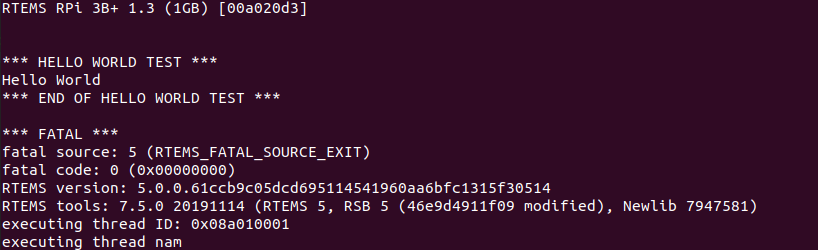
\includegraphics[scale = 0.5]{images/hello_world_log.png}
    \caption{Hello world log}
    \label{fig:hello_world_log}
\end{figure}

Il messaggio di errore su terminale è causato dalla funzione \textbf{'exit(n)'}, presente nel task Init per \textbf{terminare l'applicativo} con 'fatal code' uguale al parametro 'n'.
La funzione 'exit(n)' causa un messaggio di errore perché si prevede che un applicativo RTEMS sia sempre in esecuzione, e quindi il termine di esso per RTEMS è considerato un comportamento imprevisto.
Se non si vuole avere questo messaggio di errore bisogna inserire nel codice un ciclo infinito, in modo che il programma non termini mai.\newline
%Senza la funzione 'exit(n)' avremmo il codice di errore uguale a 5 che corrisponde ad INTERNAL\_ERROR\_THREAD\_EXITTED poiché non essendoci altre funzioni o un ciclo infinito dopo la funzione 'printf(..)', il task Init termina . 

L'\textbf{interfaccia GPIO }è stata validata con tre programmi per coprire le seguenti situazioni :
\begin{enumerate}
    \item accensione e spegnimento di un led ad intervalli di 1 secondo.
    \item alla pressione di un bottone si ha l'accensione o spegnimento di un led.
    \item alla pressione di un bottone, viene avviato un task.
\end{enumerate}

Il \textbf{primo programma} sui GPIO, il file init.c ha solo il task Init, dove è presente un ciclo infinito (while(1)) per il cambio di stato del LED e le API di RTEMS per la gestione del GPIO :
\begin{itemize}
    \item\parbox[t]{\linewidth}{rtems\_gpio\_initialize(): inizializza le API dei GPIO}
    \item\parbox[t]{\linewidth}{rtems\_status\_code rtems\_gpio\_bsp\_select\_input(uint32\_t bank,uint32\_t pin,  void *bsp\_specific): imposta il pin come input, discorso analogo l'output.}
    \item\parbox[t]{\linewidth}{uint32\_t rtems\_gpio\_bsp\_get\_value(uint32\_t bank, uint32\_t pin): recupera il valore del pin}
    \item\parbox[t]{\linewidth}{rtems\_status\_code rtems\_gpio\_bsp\_clear(uint32\_t bank, uint32\_t pin): imposta il valore del pin a 0}
    \item\parbox[t]{\linewidth}{rtems\_status\_code rtems\_gpio\_bsp\_set(uint32\_t bank, uint32\_t pin): imposta il valore del pin a 1}
\end{itemize}
\begin{lstlisting}[style = CStyle]
  ...
  rtems_interval  seconds = 1 * rtems_clock_get_ticks_per_second();
  rtems_gpio_initialize();
  rtems_gpio_bsp_select_input(0, pin, &bsp_spec);
  rtems_gpio_bsp_select_output(0, pin, &bsp_spec);
  while(1){
	  if(rtems_gpio_bsp_get_value(0, pin)){
		  rtems_gpio_bsp_clear(0,pin);
	  }else{
		  rtems_gpio_bsp_set(0,pin);
	  }
	  rtems_task_wake_after(seconds);
  }
  ...
\end{lstlisting}
\newpage
Il \textbf{secondo programma} sui GPIO ha come scopo validare anche la gestione degli interrupts. 
È un circuito elettrico per generare un interrupt tramite pulsante e vedere la gestione dallo stato di un LED.\newline
\begin{figure}[h]
\begin{subfigure}{0.5\textwidth}
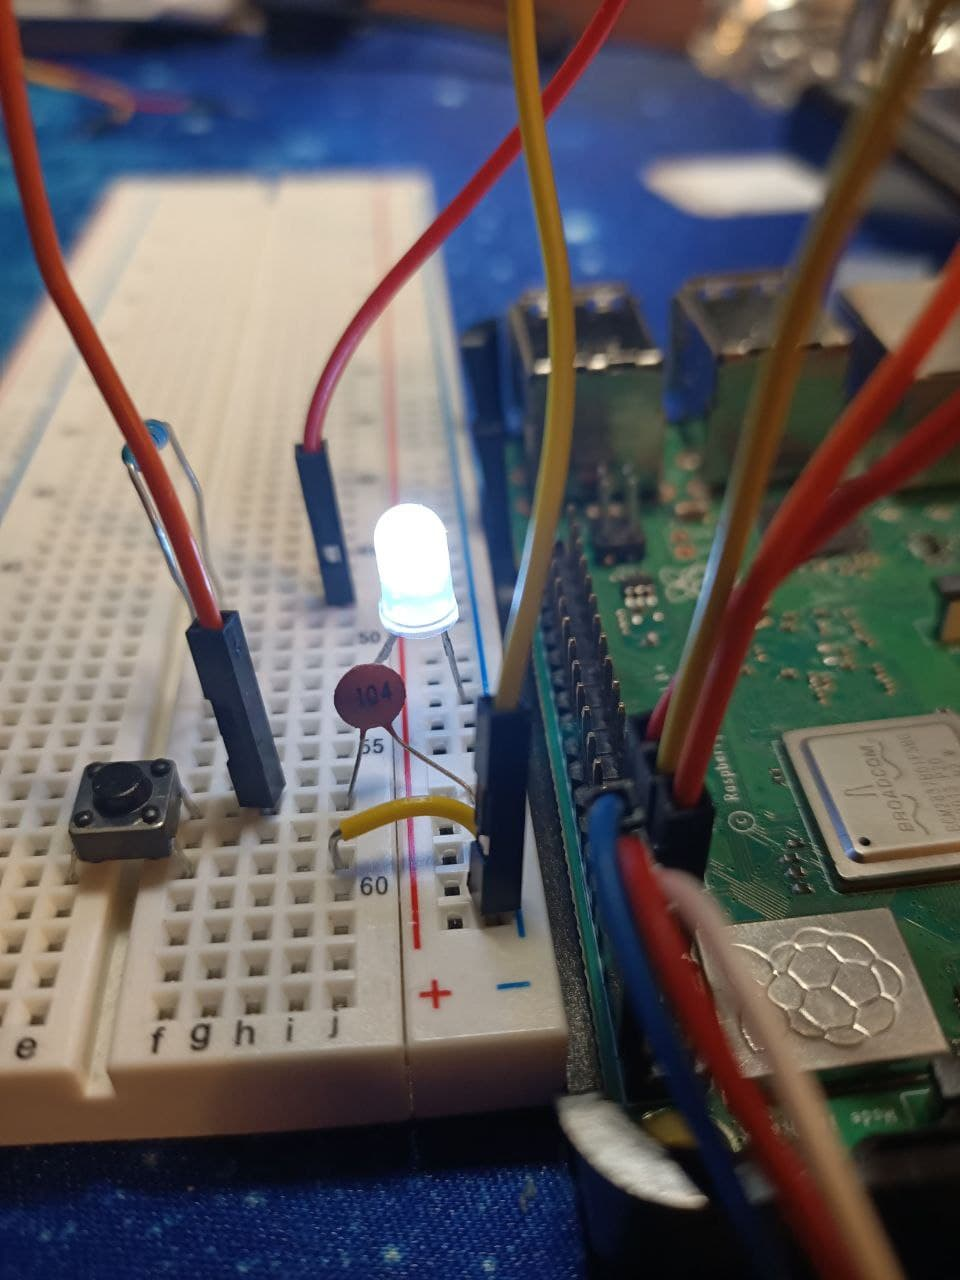
\includegraphics[width=1.2\linewidth, height=8cm]{images/Btn_switch_led_circuit_image_2.JPG}
\caption{Circuito con Raspberry Pi}
\label{fig:Circuito con Raspberry Pi}
\end{subfigure}
\begin{subfigure}{0.5\textwidth}
%TODO correggere
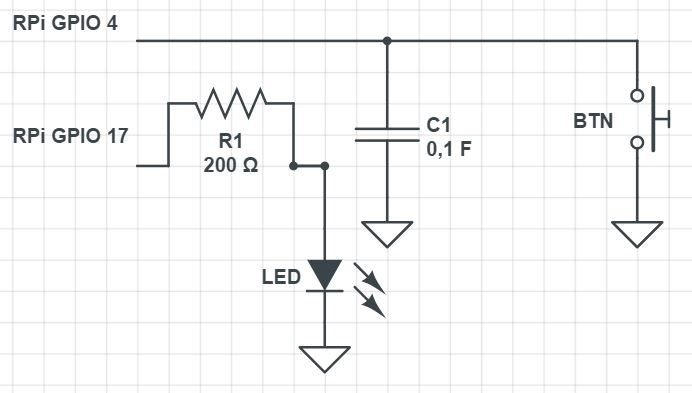
\includegraphics[width=1.2\linewidth, height=8cm]{images/Btn_switch_led_circuit_schema.JPG}
\caption{Schema elettrico del circuito}
\label{fig:Schema elettrico del circuito}
\end{subfigure}
\end{figure}
In questo programma si hanno due task, Init e ld\_switch.
Il task Init si occupa della configurazione dei GPIO e interrupts, creazione del task ld\_switch, creazione del semaforo e avvio del ld\_switch.
Il task ld\_switch è quello che esegue il cambio di stato del LED che dipende dallo stato del pulsante gestito da interrupt.
Per la configurazione degli interrupt vengono utilizzate le API di RTEMS generiche :
\begin{itemize}
    \item rtems\_status\_code rtems\_gpio\_resistor\_mode(
  uint32\_t pin\_number,
   rtems\_gpio\_pull\_mode mode
) : imposta in pull-up o pull-down la resistenza del pin
    \item rtems\_status\_code rtems\_gpio\_enable\_interrupt(
  uint32\_t pin\_number,
  rtems\_gpio\_interrupt interrupt,
  rtems\_gpio\_handler\_flag flag,
  bool threaded\_handling,
  rtems\_gpio\_irq\_state (*handler) (void *arg),
  void *arg
) : abilita l'interrupt sul pin, e assegna l'handler già definito.
    \item rtems\_status\_code rtems\_gpio\_debounce\_switch(
  uint32\_t pin\_number,
  int ticks
) : imposta il tempo del 'debounce' del pin.
\end{itemize}
Tra l'handler dell'interrupt e il task ld\_switch si verifica il problema della gestione della \textbf{sezione critica} sulla variabile dello stato del pulsante, ciò è stata risolta utilizzando gli \textbf{eventi} e un \textbf{semaforo binario}.\newline
Per utilizzare i semafori è necessario aggiungere una direttiva in più "CONFIGURE\_MAXIMUM\_SEMAPHORES " impostando il numero massimo di semafori consentiti, in questo caso 1. \newline
Di seguito il codice in cui viene gestita la sezione critica:
\begin{lstlisting}[style = CStyle]
rtems_gpio_irq_state btn_handler(void *arg) {
	sem_status = rtems_semaphore_obtain(sem_id,RTEMS_WAIT, RTEMS_NO_TIMEOUT);
	if(sem_status != RTEMS_SUCCESSFUL){
		print_to_console_error("rtems_sem_obt failed ", sem_status);
		exit(sem_status);
	}
	//send event to ld_switch task
	rtems_event_send(tid_1, RTEMS_EVENT_0);
	if(get_ld_status()){
		set_ld_status(false);
	}else{
		set_ld_status(true);
	}
	rtems_semaphore_release(sem_id);
	return IRQ_HANDLED;
}
rtems_task ld_switch(rtems_task_argument sec){
	print_to_console("initialized btn_polling_task \n");
	rtems_event_set event_out;
	while(1){
		//wait until btn_interrupt send event
		rtems_event_receive(RTEMS_EVENT_0, RTEMS_WAIT, RTEMS_NO_TIMEOUT, &event_out);
		//wait until btn_interrupt release semamphore
		sem_status = rtems_semaphore_obtain(sem_id, RTEMS_WAIT, RTEMS_NO_TIMEOUT);
		if(sem_status != RTEMS_SUCCESSFUL){
			print_to_console_error("rtems_sem_obt failed ", sem_status);
			exit(sem_status);
		}
		if(get_ld_status()){
			rtems_gpio_bsp_set(0, ld_pin);
			print_to_console("1");
		}else{
			rtems_gpio_bsp_clear(0, ld_pin);
			print_to_console("0");
		}
		rtems_semaphore_release(sem_id);
	}
}
\end{lstlisting}

\newpage
Il \textbf{terzo programma} è composto da due task oltre il task Init:
\begin{itemize}
    \item \textbf{btn\_polling} : controlla la variabile di stato del pulsante, se risulta true (quindi è stato  premuto), allora viene avviato il task led\_blink.
    \item \textbf{led\_blink} : accende o spegne 3 volte il LED con un intervallo di tempo di 1 secondo.
\end{itemize}
Il circuito elettrico è lo stesso del programma precedente.
Anche in questo programma è presente la sezione critica per la variabile di stato del pulsante, e viene gestita nello stesso modo.
In questo caso bisogna modificare lo stato dei task in modo da non farli interferire tra loro.\newline
\begin{figure}[h]
    \centering
    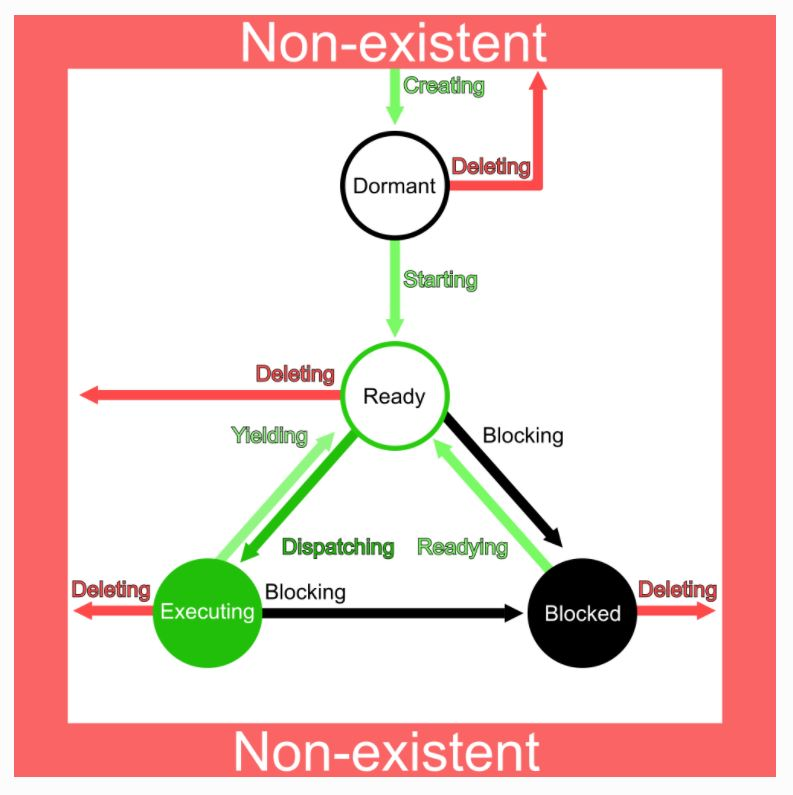
\includegraphics[scale = 0.5]{images/task_state.JPG}
    \caption{Stato dei task}
    \label{fig:Stato dei task}
\end{figure}
Il task Init dopo aver configurato l'applicativo e creato i task, avvia il task "btn\_polling" che passa dallo stato 'Ready' allo stato 'Executing'.
Il task "btn\_polling" quando riceve riceve l'evento dall'handler interrupt avvia il task "ld\_blink" cambiandogli stato da 'Ready' a 'Executing' con l' API rtems\_task\_restart(..) oppure rtems\_task\_start(..), ciò dipende se il task era in stato 'Blocked'. Inoltre viene cambiato lo stato del task btn\_polling in 'Blocked' con l'API rtems\_task\_suspend(..).\newline
In questo modo rimane in esecuzione solo il task ld\_blink, che come ultime operazioni ha il  ripristino dell'esecuzione del task btn\_polling con l'API rtems\_task\_resume e quindi viene cambiato lo stato in 'Executing' e viene sospeso il task ld\_blink.\newline
Seguendo questi passaggi rimane in esecuzione solo un task alla volta.
%Il task Init dopo aver configurato il sistema e creato i task, avvia il task btn\_polling.
\newpage
\begin{lstlisting}[style = CStyle]
...
rtems_task btn_task(rtems_task_argument sec){
	print_to_console("initialized btn_polling_task \n");
	rtems_event_set event_out;
	while(1){
		rtems_event_receive(RTEMS_EVENT_0, RTEMS_WAIT, RTEMS_NO_TIMEOUT, &event_out);
		sem_status = rtems_semaphore_obtain(sem_id, RTEMS_WAIT, RTEMS_NO_TIMEOUT);
			if(btn_status == true){
				status_1 = rtems_task_restart( tid_2, 0);
				if ( status_1 == RTEMS_INCORRECT_STATE ) {
					rtems_task_start(tid_2,ld_blink,0);
			   }else if (status_1 != RTEMS_SUCCESSFUL){
				   print_to_console_error("ld_blink_task start failed ", status_1);
			   }
				rtems_task_suspend(tid_1);
				btn_status = false;
			}
		rtems_semaphore_release(sem_id);
	}
}
rtems_task ld_blink(rtems_task_argument null){
	rtems_interval two_sec = 2 * rtems_clock_get_ticks_per_second();
	uint32_t count = 0;
	print_to_console("initialized ld_blink_task \n");
	while(count<4){
		if(rtems_gpio_bsp_get_value(0, ld_pin)){
			rtems_gpio_bsp_clear(0, ld_pin);
		}else{
			rtems_gpio_bsp_set(0, ld_pin);
			count++;
		}
		rtems_task_wake_after(two_sec);
	}
	btn_status=false;
	rtems_task_resume(tid_1);
	rtems_task_suspend(tid_2);
}
\end{lstlisting}
\newpage
Per l'interfaccia \textbf{I2C} è stato creato un programma che legge l'output del componente ADC che ,manipolandolo come indicato dal datasheet, da come risultato la tensione in entrata al ADC. Poiché bisogna utilizzare un componente aggiuntivo, ho dovuto creare il driver associato.\newline
Il driver è composto da due file sorgenti:
\begin{itemize}
    \item \textbf{mcp3425.h}: in questo file viene dichiarata la funzione \textbf{int i2c\_dev\_register\_\newline mcp3425 (const char *bus\_path, const char *dev\_path, uint16\_t address);} che serve per configurare il bus I2C ed associare il file in dev\_path all'indirizzo di periferica address.
    Questo file header deve essere inserito nella cartella libchip, che contiene tutti i file header dei driver .
    \item \textbf{mcp3425.c}: in questo file viene definita la funzione dichiarata in "mcp3425.h", e i comandi ioctl che verranno utilizzato nel programma.
\end{itemize}

La funzione \textbf{i2c\_dev\_register\_mcp342}5 è così definita:
\begin{lstlisting}[style = CStyle]
int i2c_dev_register_mcp3425(const char *bus_path, const char *dev_path, uint16_t address) {
  i2c_dev *dev;
  dev = i2c_dev_alloc_and_init(sizeof(*dev), bus_path, address);
  if (dev == NULL) {
	  printf("error code %u from i2c_dev_alloc_and_init(..) \n", errno);
	  fflush(stdout);
	  return -1;
  }
  dev->ioctl = i2c_mcp3425_linux_ioctl;
  return i2c_dev_register(dev, dev_path);

}
\end{lstlisting}
L' API di RTEMS \textbf{i2c\_dev\_alloc\_and\_init} serve ad inizializzare e associare il 'device control' all'indirizzo di periferica passato come parametro in input. Successivamente viene assegnato al campo \textbf{ioctl} la funzione \textbf{i2c\_mcp3425\_linux\_ioctl} che contiene i comandi per la gestione del componente.

\newpage
I comandi ioctl vengono così definiti: 
\begin{lstlisting}[style = CStyle]
static int i2c_mcp3425_linux_ioctl(i2c_dev *dev, ioctl_command_t command, void *arg) {
  uint8_t data [2] = {0};
  int rv = 0;
  switch (command) {
    case MCP3425_CONFIG:
      rv = i2c_mcp3425_write(dev, MCP3425_REG_CONF, 0x10);
      break;
    case MCP3425_READ:
      rv = i2c_mcp3425_read(dev, MCP3425_REG_IODIR, data);
      if(rv < 0){
    	  printf("read failed %d \n", rv);
    	  fflush(stdout);
    	  return rv;
      }
      uint16_t raw_adc = ((data[0] & 0x0F) * 256 + data[1]);
      		if(raw_adc > 2047)
      		{
      			raw_adc -= 4095;
      		}
      printf("value = %d\n", raw_adc);
      return rv;
      break;
    default:
      rv = -1;
  }
  return rv;
}
\end{lstlisting}
La funzione \textbf{i2c\_mcp3425\_linux\_ioctl}gestisce due comandi che possono essere passati come parametro in input e sono "\textbf{MCP3425\_CONFIG}", per cambiare la configurazione, e "\textbf{MCP3425\_READ}" per eseguire una lettura.\newline
\newpage
Il comando \textbf{"MCP3425\_READ"} utilizza la funzione \textbf{i2c\_mcp3425\_read} che valorizza l'array data[2] con i due byte ricevuti eseguiti in lettura ed è così definita: 
\begin{lstlisting}[style = CStyle]
static int i2c_mcp3425_read(i2c_dev *dev,  uint8_t reg,  uint8_t* reg_content) {
  i2c_msg msg [2] = {
    {
    .addr = dev->address,
    .flags = 0,
    .len = 1,
    .buf = &reg
    },
    {
    .addr = dev->address,
    .flags = I2C_M_RD,
    .len = 2,
    .buf = reg_content
    }
  };
  return i2c_bus_transfer(dev->bus, msg, 2);
}
\end{lstlisting}
In questa funzione creiamo due \textbf{i2c\_msg}, una struttura che definisce i messaggi i2c da trasmettere, che verrano passati come parametro al'API \textbf{i2c\_bus\_transfer(...)}.\newline
Al termine della lettura dei due byte, vengono eseguite delle operazioni sui bit dell'array data[2] in modo da escludere i 4 most significant bit ed avere il risultato in 16 bit.\newline
Il comando ioctl "MCP3425\_CONFIG" non viene utilizzato, ma viene inserito solo per rendere completo il driver, e serve a cambiare la configurazione del componente.\newline
\newpage
Per eseguire le funzioni di lettura e scrittura devono essere invocate dal task Init utilizzando la 'system call' \textbf{ioctl}(int fd, long request, ...), che serve a fare operazioni su file che rappresentano i punti di accesso alle periferiche, nel mio caso il file è "/dev/i2c-1.mcp3425". \newline
La funzione open(...) recupera il file descriptor che identifica il punto di accesso, ed è il parametro in input ("fd")  nella funzione ioctl(int fd, long request), dove la request è un enum che rappresenta il comando ioctl del driver .\newline
\begin{lstlisting}[style = CStyle]
    ...
	int rv = i2c_dev_register_mcp3425("/dev/i2c-1", "/dev/i2c-1.mcp3425", MCP3425_ADDR);
	if(rv < 0){
		exit(errno);
	}
	printf("mcp34225 registration success\n");
	fflush(stdout);
	int fd = open("/dev/i2c-1.mcp3425", O_RDWR);
	if(fd < 0){
		printf("error open mcp3425 %u \n", errno);
		fflush(0);
		exit(errno);
	}
	printf("i2c.mcp3425 open success\n");
	fflush(stdout);
	...
	int count = 0;
	while(1 && count < 3){
		ioctl(fd, MCP3425_READ,NULL);
		rtems_task_wake_after(1*rtems_clock_get_ticks_per_second());
		count++;
	}
	rv = close(fd);
\end{lstlisting}

\newpage
Per l'interfaccia \textbf{SPI} è stato creato un programma in cui si effettua cinque volte la scrittura di un valore, da 0 a  4095, sul componente DAC che a sua volta restituisce come output la tensione risultante dalla conversione. Anche in questo caso si è dovuto creare il driver associato \newline
Il driver è composto da due file sorgenti:
\begin{itemize}
    \item\textbf{mcp4822.h}: in questo file header viene dichiarata la funzione \textbf{int spi\_libi2c\_ \newline register\_mcp4822(unsigned spi\_bus)}; che serve per configurare il bus SPI, inizializzare il driver ed associarlo al pin di selezione CE0.
    Questo file header deve essere inserito nella cartella libchip.
    \item\textbf{mcp4822.c}: in questo file viene definita la funzione dichiarata sul file header mcp4822.h, ed anche la funzione di scrittura sul componente che verrà utilizzata.
\end{itemize}

La funzione spi\_libi2c\_register\_mcp4822 viene così definita:
\begin{lstlisting}[style = CStyle]
static rtems_driver_address_table spi_mcp4822_rw_ops = {
  .read_entry = spi_mcp4822_read,
  .write_entry = spi_mcp4822_write
};

static rtems_libi2c_drv_t spi_mcp4822_rw_drv_t = {
  .ops = &spi_mcp4822_rw_ops,
  .size = sizeof(spi_mcp4822_rw_drv_t)
};

int spi_libi2c_register_mcp4822(unsigned spi_bus)
{
  return rtems_libi2c_register_drv(
           "mcp4822",
           &spi_mcp4822_rw_drv_t,
           spi_bus,
           SPI_MCP4822_ADDR
         );
}
\end{lstlisting}
L'API \textbf{rtems\_libi2c\_register\_drv} assegna al file "mcp4822" la driver table \newline "spi\_mcp4822\_rw\_drv\_t", il bus spi già inizializzato e passato come parametro in input, e il pin di selezione "SPI\_MCP\_4822\_ADDR". Se il valore della macro SPI\_MCP\_4822\_ADDR è pari a 0 allora il driver viene associato al pin CE0, analogamente se il valore della macro è pari a 1.\newline
Nella driver table vengono assegnate le operazioni tramite la 'rtems\_driver\_address\_table' \textbf{spi\_mcp4822\_rw\_ops} che definisce le entry point per la scrittura e lettura.\newline
Il componente ha una comunicazione unidirezionale, per questo motivo nella funzione  "spi\_mcp4822\_read" non viene fatta nessuna operazione ma viene restituito lo status code RTEMS\_NOT\_CONFIGURED.\newline
Invece all'entry point della scrittura vien associata la funzione "\textbf{spi\_mcp4822\_write}" ed è così definita:\newline
\begin{lstlisting}[style = CStyle]
...
static rtems_status_code spi_mcp4822_write(rtems_device_major_number major, rtems_device_minor_number minor, void *arg) {
	rtems_status_code sc = RTEMS_SUCCESSFUL;
	rtems_libio_rw_args_t *rwargs = arg;
	int cnt = rwargs -> count;
	unsigned char *buf = (unsigned char *) rwargs -> buffer;
	/*send start*/
	sc = rtems_libi2c_send_start(minor);
	if(sc<0){
		printf("send start error \n");
		fflush(stdout);
		return sc;
	}else{
		printf("start sended \n");
		fflush(stdout);
	}
	/*set ioctl transfer mode*/
	sc = rtems_libi2c_ioctl(minor, RTEMS_LIBI2C_IOCTL_SET_TFRMODE, &tfr_mode);
	 if ( sc != RTEMS_SUCCESSFUL ) {
		printf("ioctl error \n");
		fflush(stdout);
	    return sc;
	 }else{
		printf("ioctl setted \n");
		fflush(stdout);
	 }
	/*send addr*/
	sc = rtems_libi2c_send_addr(minor, TRUE);
    if ( sc != RTEMS_SUCCESSFUL ) {
      printf("send address error \n");
	  fflush(stdout);
      return sc;
    }else{
		printf("address sended \n");
		fflush(stdout);
    }
	/*write bytes*/
	int data_sent_cnt = rtems_libi2c_write_bytes(minor, buf, cnt);
    if (data_sent_cnt < 0) {
	  printf("write bytes error \n");
	  fflush(stdout);
      return RTEMS_IO_ERROR;
    }else{
      printf("wrote %d bytes \n", data_sent_cnt);
      fflush(stdout);
    }
	/*send stop*/
	sc = rtems_libi2c_send_stop(minor);
    if ( sc != RTEMS_SUCCESSFUL ) {
	  printf("send stop error \n");
	  fflush(stdout);
      return sc;
    }else{
		printf("stop sended \n");
		fflush(stdout);
    }
	return RTEMS_SUCCESSFUL;
}
...
\end{lstlisting}
In questa funzione viene utilizzata la libreria  generica per la gestione del I2C e del SPI, \textbf{libi2c}.\newline
Per un corretto utilizzo delle API libi2c è necessario seguire un ordine preciso con cui vengono usate:
\begin{enumerate}
    \item \textbf{rtems\_libi2c\_send\_start}: blocca l'accesso al SPI bus alle altre periferiche, viene creata una mutua esclusione. Se si vuole utilizzare il bus SPI con altre periferiche bisogna utilizzare l'api "rtems\_libi2c\_send\_stop".
    \item \textbf{rtems\_libi2c\_ioct}l: serve ad effettuare operazioni ioctl sul componente. In questo caso viene usato per impostare le specifiche di trasferimento dei dati, ad esempio il baudrate.
    \item \textbf{rtems\_libi2c\_send\_addr}: attiva il pin di selezione associato al componente, in questo caso il pin CE0.
    \item \textbf{rtems\_libi2c\_write\_bytes}: effettua la scrittura dei byte sul componente
    \item \textbf{rtems\_libi2c\_send\_stop}: disattiva il pin di selezione e sblocca il bus SPI, in modo da poter essere utilizzato con altre periferiche.
\end{enumerate}
\newpage
La funzione rtems\_libi2c\_ioctl ha come parametro in input il  "\&tfr\_mode", ed è un struttura che definisce la modalità di trasferimento dei dati:
\begin{lstlisting}[style = CStyle]
static rtems_libi2c_tfr_mode_t tfr_mode = {
  .baudrate = 20000000,
  .bits_per_char = 8,
  .lsb_first = FALSE,
  .clock_inv = TRUE,
  .clock_phs = FALSE
};
\end{lstlisting}
Questa struttura viene definita facendo riferimento alle specifiche del componente, che si possono trovare nel datasheet \cite{microchipMCP4822}
\section{Risultati finali}

Le applicazioni real-time oltre al risultato devono rispettare dei tempi stabiliti, per questo motivo viene utilizzato un \textbf{oscilloscopio} per generare dei grafici qualitativi dei segnali prodotti dal software, su tutti gli applicativi RTEMS creati. Quindi con lo stesso ordine con cui vengono esposti i programmi nel capitolo precedente, viene fatta un'analisi delle forme d'onda di ogni programma\newline
Il \textbf{primo programma} di validazione dell'interfaccia \textbf{GPIO}, che esegue l'accensione e spegnimento di un led ad intervalli di 1 secondo, genera la seguente forma d'onda:\newline
\begin{figure}[h]
    \centering
    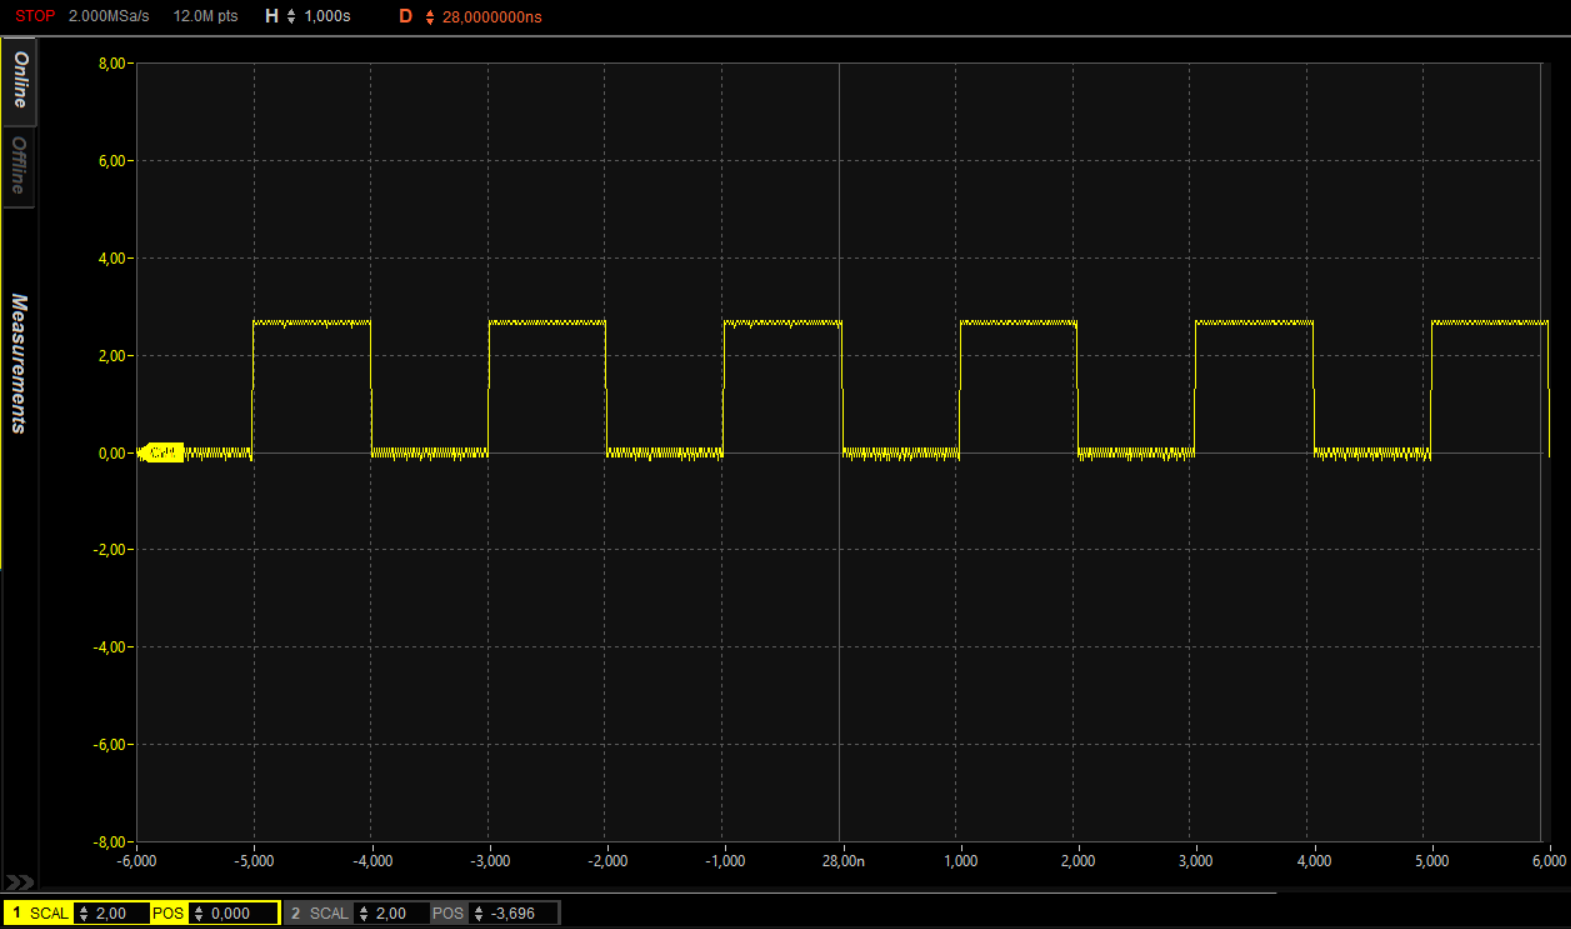
\includegraphics[scale = 0.40]{images/led_graph/LED_BLINK_5.PNG}
\end{figure}
\newpage 
Si può notare che il LED rimane precisamente in uno livello alto o basso per 1 secondo.\newline
Cambiando l'impostazione dell'asse orizzontale, che rappresenta la base tempi, si può visualizzare con dettaglio il cambio di stato del LED:
\begin{figure}[h]
    \centering
    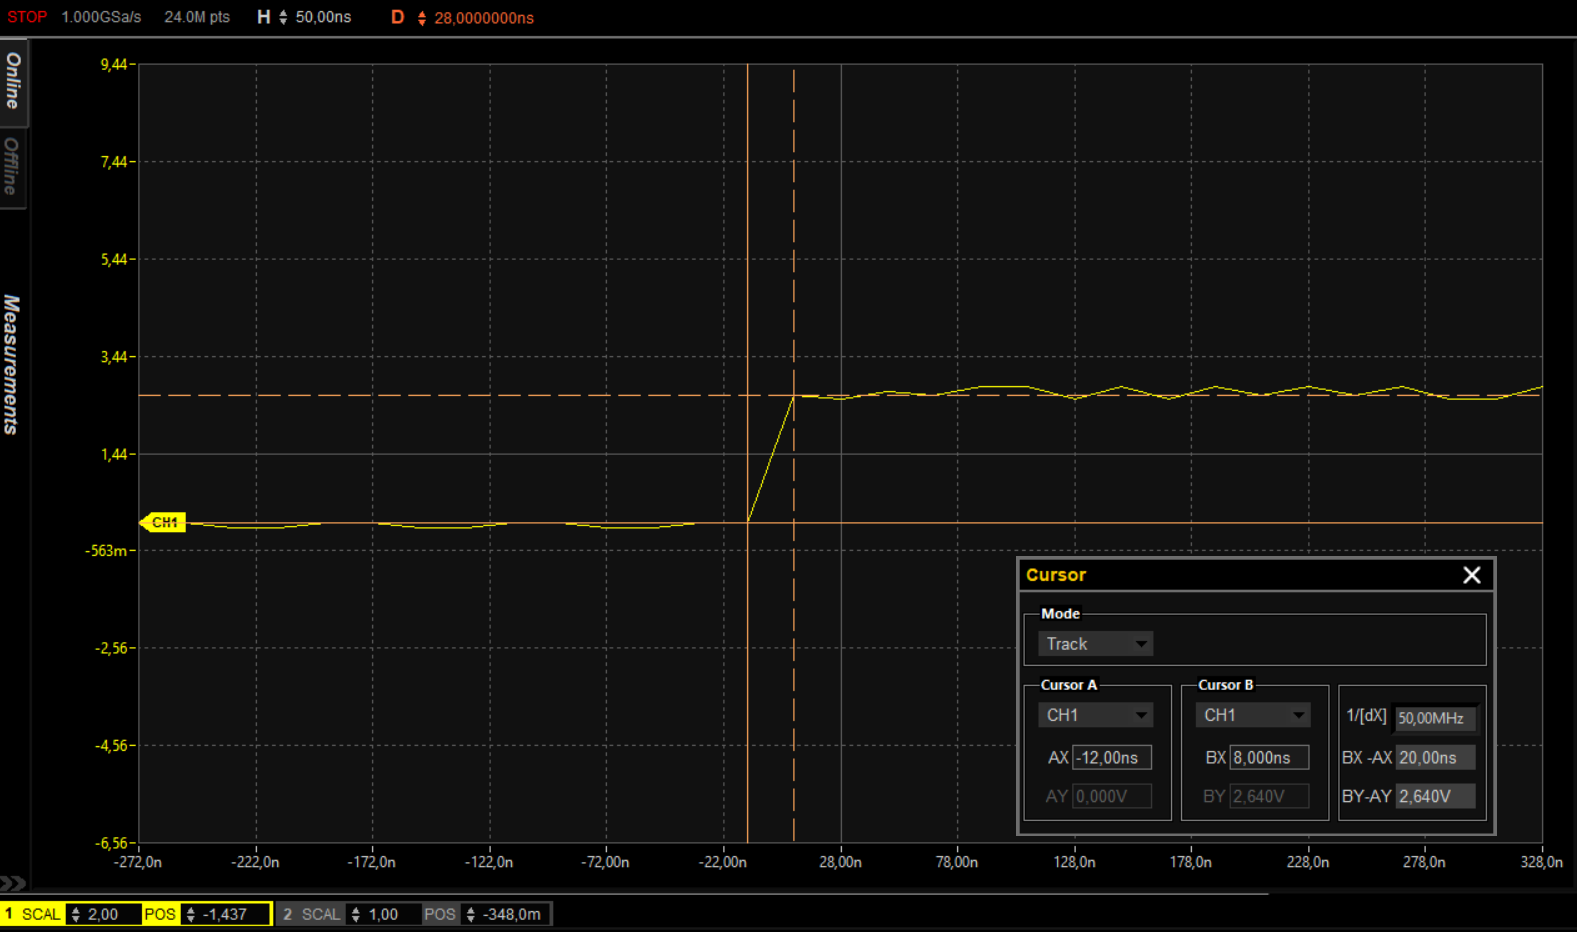
\includegraphics[scale = 0.40]{images/led_graph/LED_BLINK_4.PNG}
\end{figure}
\newline
Si nota che il cambio di stato del LED richiede 20ns.\newline
Il \textbf{secondo programma} per l'interfaccia \textbf{GPIO}, in cui viene generato un interrupt tramite pulsante per cambiare lo stato di un LED, genera la seguente forma d'onda:\newline
\begin{figure}[h]
    \centering
    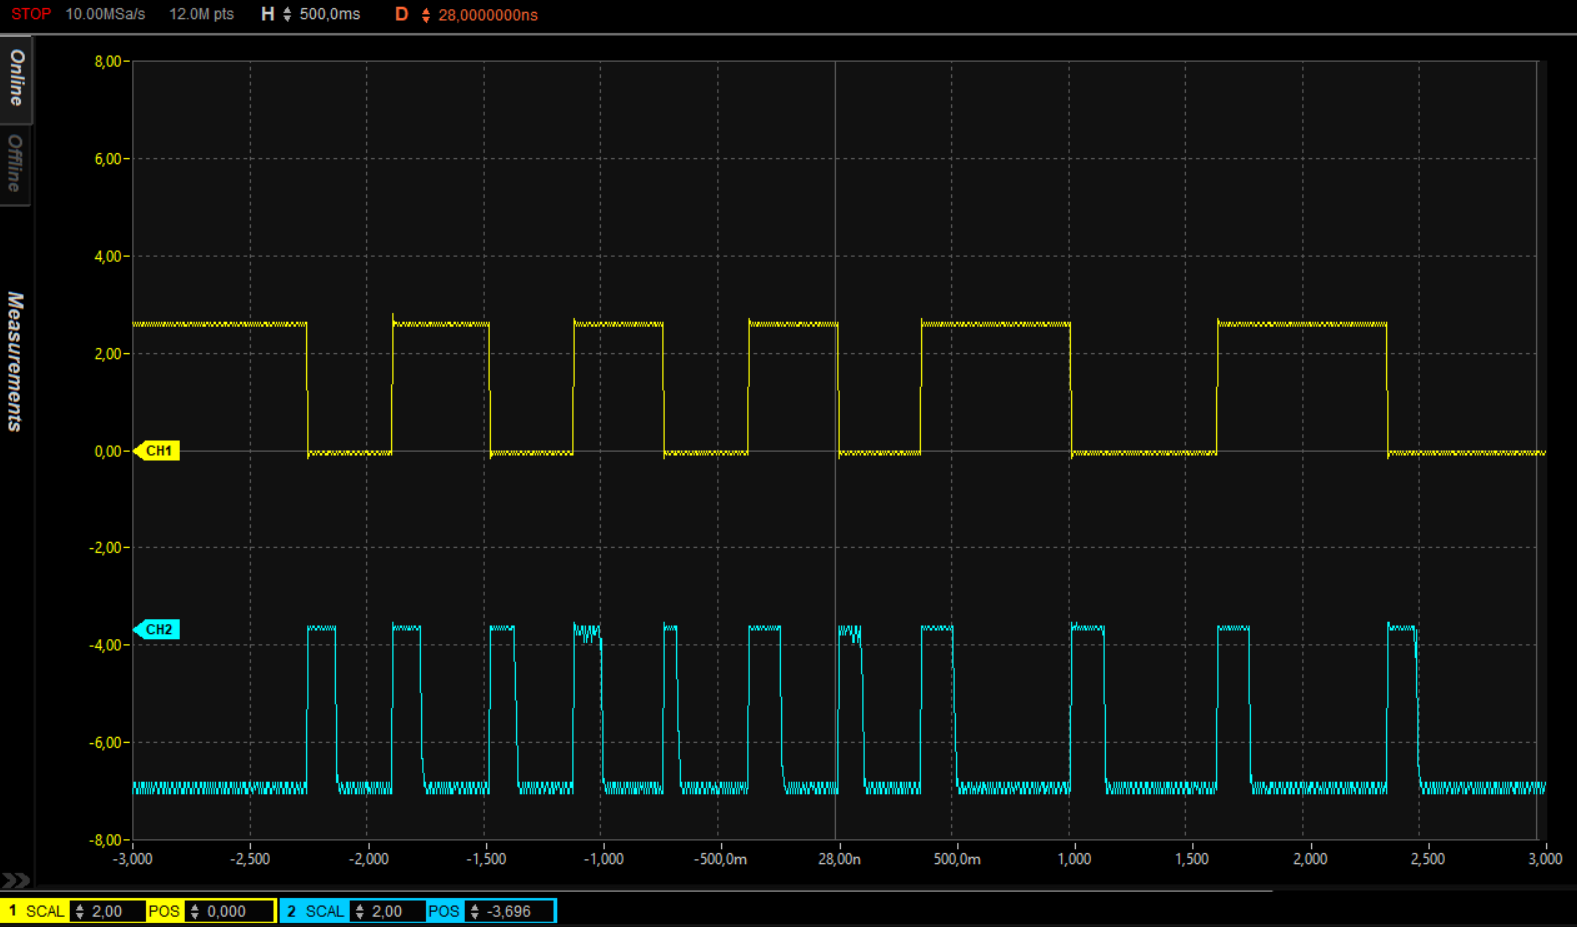
\includegraphics[scale = 0.40]{images/btn_switch_graph/BTN_SWITCH_5.PNG}
    \caption{Forme d'onda che rappresentano LED e pulsante}
    \label{fig:btn_1}
\end{figure}
\newline
Vengono usati due canali dove il primo (in giallo) rappresenta la tensione del LED, invece il secondo canale (in azzurro) rappresenta la tensione invertita del pulsante.
Anche in questo caso viene impostata la base tempi per avere in dettaglio il tempo che trascorre tra l'interrupt e l'accensione o spegnimento del LED:
\newline
\begin{figure}[h]
    \centering
    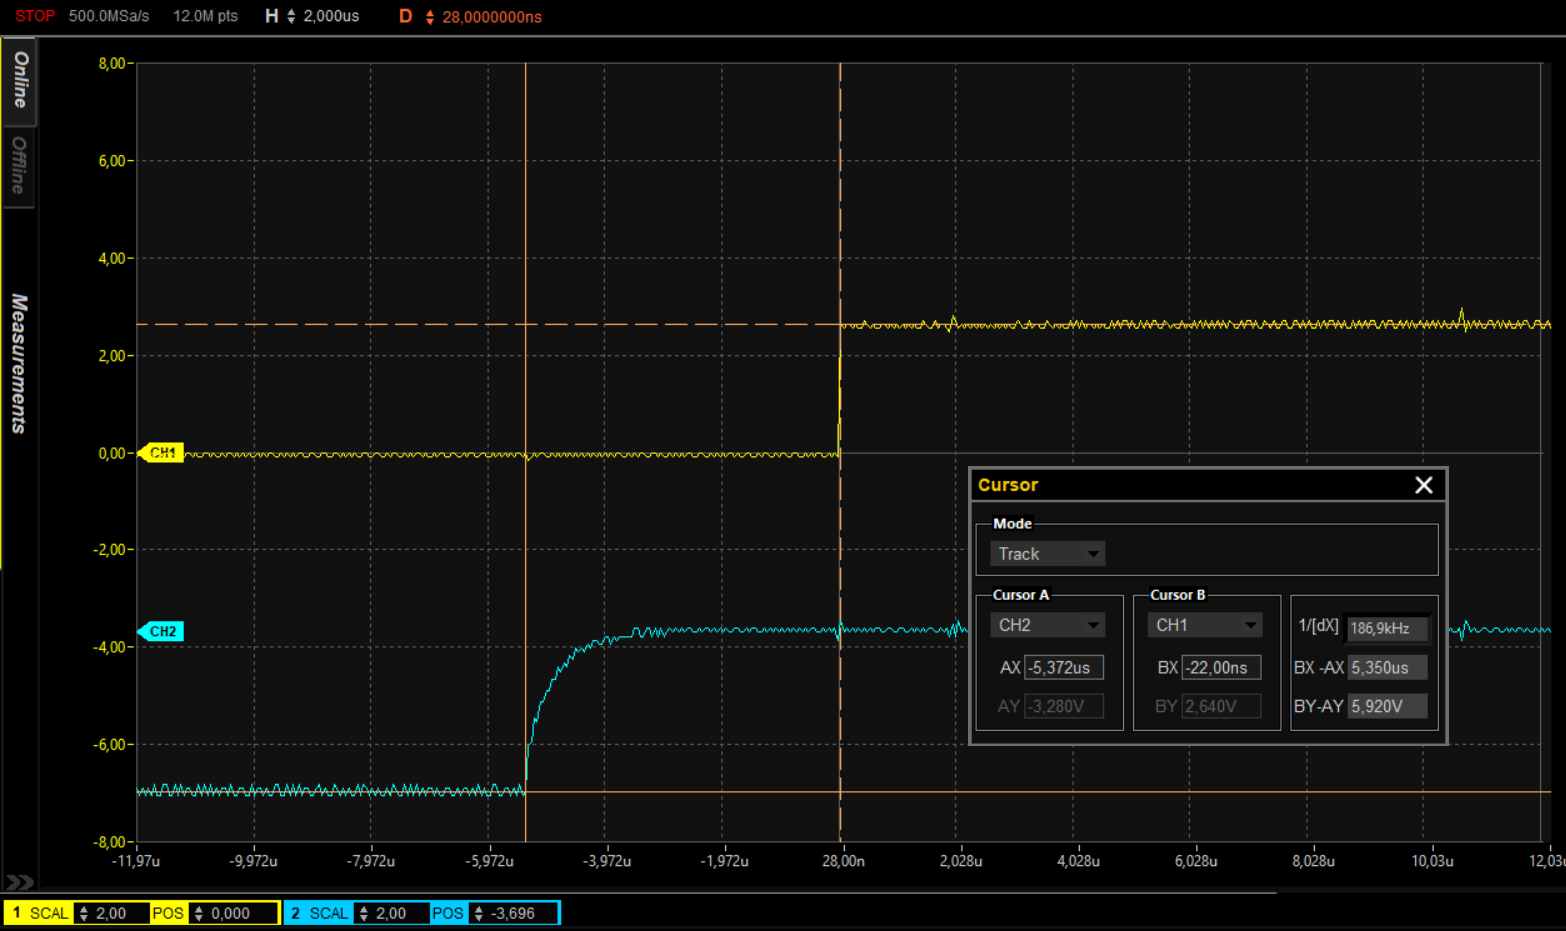
\includegraphics[scale = 0.40]{images/btn_switch_graph/BTN_SWITCH_4.PNG}
    \caption {generazione dell'interrupt e il cambio di stato del LED in dettaglio}
    \label{fig:btn_2}
\end{figure}
\newline
Utilizzando i cursori in dotazione nell'oscilloscopio, si nota che il cambio di stato del led richiede 5.350us dall'interrupt.\newline
\newpage
L'\textbf{ultimo programma di validazione} dell'interfaccia \textbf{GPIO}, in cui viene generato un interrupt per avviare un task genera un grafico simile al precedente programma, con la sola differenza che dopo aver fatto scattare l'interrupt lo stato del LED cambia 6 volte ogni 2 secondi per poi rimanere a livello alto in attesa di un ulteriore interrupt.\newline
\begin{figure}[h]
    \centering
    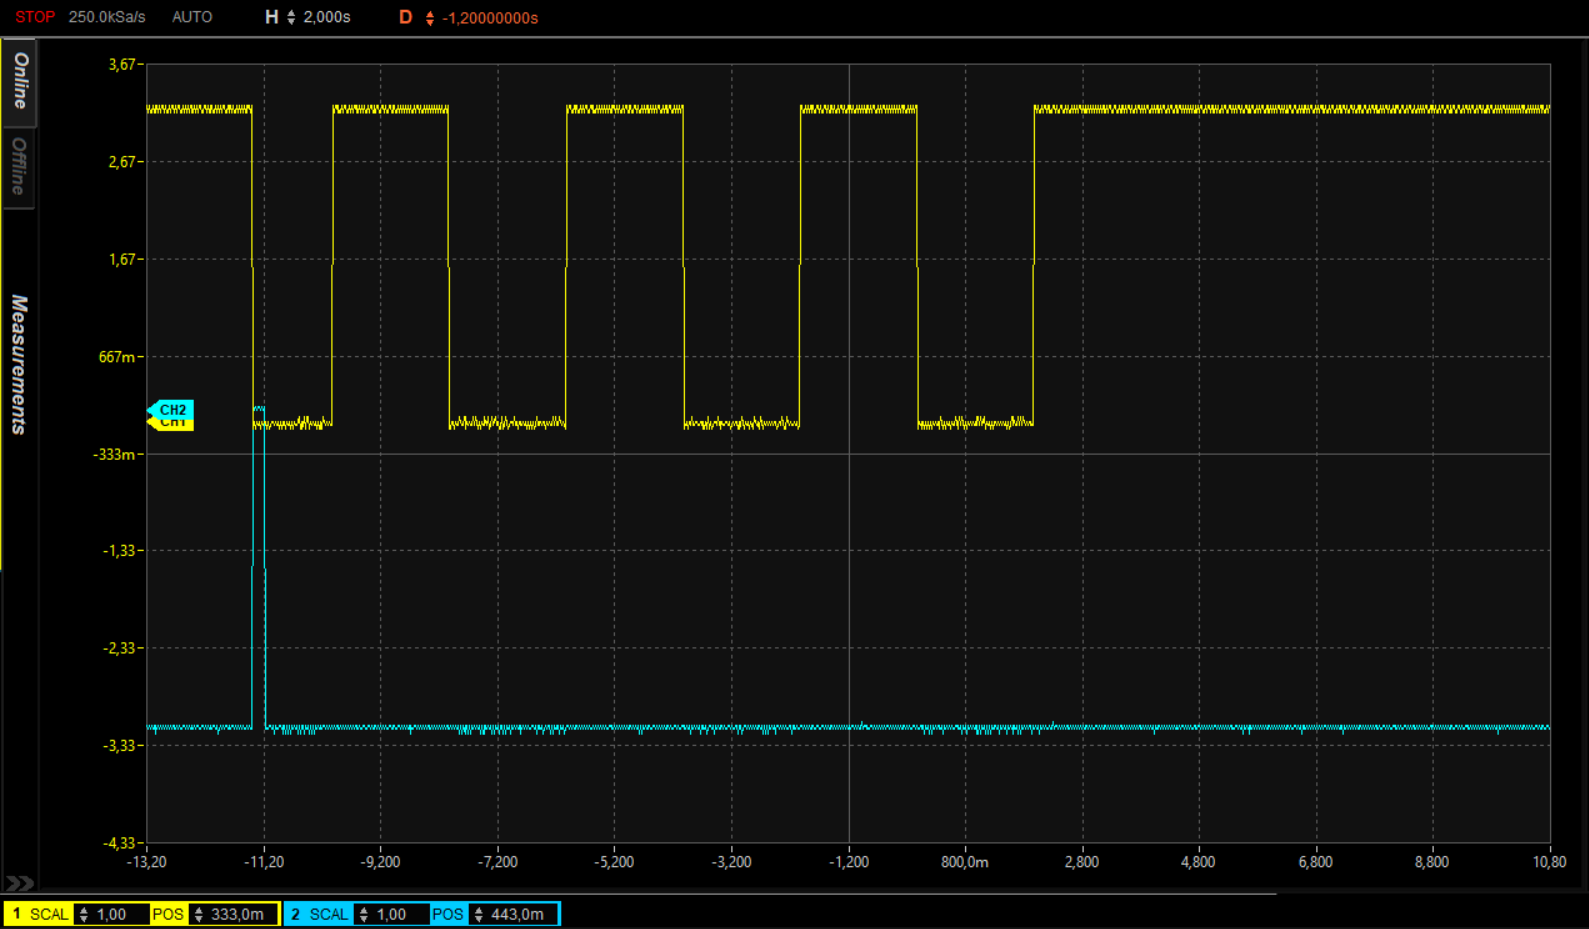
\includegraphics[scale = 0.40]{images/btn_switch_graph/BTN_START_TASK.PNG}
        \caption{Forme d'onda che rappresentano MOSI e CS}
    \label{fig:gpio_graph2}
\end{figure}

I programmi di validazione più complessi sono state le interfacce \textbf{I2C} e \textbf{SPI}, poiché richiedevano la creazione dei driver per i componenti aggiuntivi.\newline
Per la creazione dei driver vengono presi come riferimento i programmi di test dati a disposizione dall'ing. Marques, nel suo Git repository pubblico \cite{asuol}.\newline
Durante la creazione del programma per l'I2C, il primo problema è stato l'utilizzo di un bus path errato, ciò causava un errore in run-time durante l'inizializzazione del bus. Dopo aver individuato ed impostato il bus path corretto, l'applicativo non dava più errori in run-time ma rimaneva bloccato sull'operazione di lettura.\newline
A questo punto è stata aperta una 'issue' sul Git repository dell'ing. Marques, per poter chiedere più informazioni riguardo le API per l'I2C. L'ing. Marques ha fatto notare che i cavetti che collegano la Raspberry Pi al componente MCP3425 non devono essere più lunghi di 20cm, per evitare che i dati vengano persi durante la comunicazione per via di un alta impedenza. Questo causerebbe un attesa infinita della Raspberry Pi per via della mancata ricezione dei byte. \newpage
Infatti sostituendo i cavetti si è riuscito ad effettuare le letture desiderate sul componente.\newline
Abbiamo potuto verificare anche utilizzando l'oscilloscopio ed il grafo ricavato è il seguente:\newline
\begin{figure}[h]
    \centering
    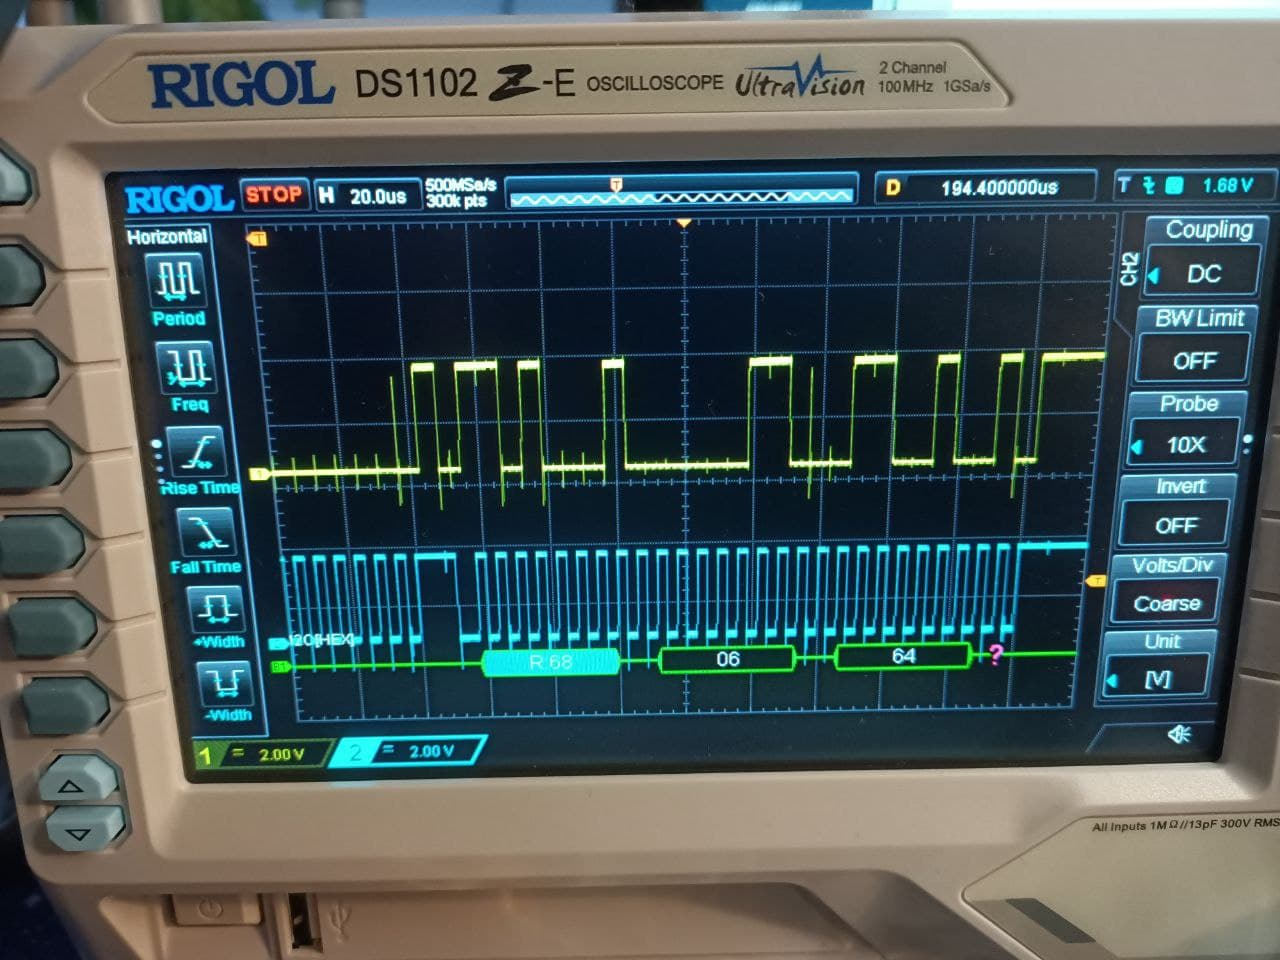
\includegraphics[scale =0.30]{images/i2c_graph/I2C_oscilloscopio.jpg}
    \caption{Forme d'onda che rappresentano SDA e SCKL}
    \label{fig:I2C_graPH}
\end{figure}
\newline
Il canale 1, in giallo, rappresenta la forma d'onda del pin 'SDA' dove riceviamo i bit che leggere dal componente.
Invece canale 2, in blu, rappresenta la forma d'onda del pin 'SCKL'.\newline
L'oscilloscopio ha incorporato un decoder I2C ed è stato utilizzato per visualizzare i dati che vengono trasmessi, in questo caso si ha come risultato: 'R:68 06 64'. \newline
'R:68' indica che l'operazione decodificata è un'operazione di lettura, i restanti dati rilevati '06 64' sono i bit che la Raspberry Pi sta ricevendo dal MCP3425 in formato esadecimale .\newline
Questi bit devono essere gestiti come scritto sul datasheet \cite{microchipMCP3425}, cioè non bisogna tenere conto dei primi 4 'most significant bit', "mascherando" il primo byte con 0x0F e poi convertire i 2 byte in decimale, come risultato deve dare la tensione del pin $V_{in+}$ dsel MCP3425.\newline
Quindi da 0x0664 ottengo il valore 1634 che corrisponde alla tensione in input del $V_{in+}$.\newline
Il programma di validazione del SPI sembra funzionare, perchè non vengono rilevati errori sul terminale e l'esecuzione non viene mai bloccata, ma l'output del canale 'A'  misurato con il multimetro risulta sempre 0V, come se la scrittura non venisse eseguita.\newline
È stato contattato l'ing. Kubler per chiarire le specifiche del componente, ed i requisiti che il software deve rispettare per effettuare la scrittura del dato, cioè che il pin di selezione deve essere a livello basso durante la scrittura, e alla fine ritornare alto per segnalare la fine della trasmissione dei dati, come mostrato nella figura 4.7 .\newline
La verifica dei requisiti è stata fatta utilizzando l'oscilloscopio che da le seguenti forme d'onda:\newline
\begin{figure}[h]
    \centering
    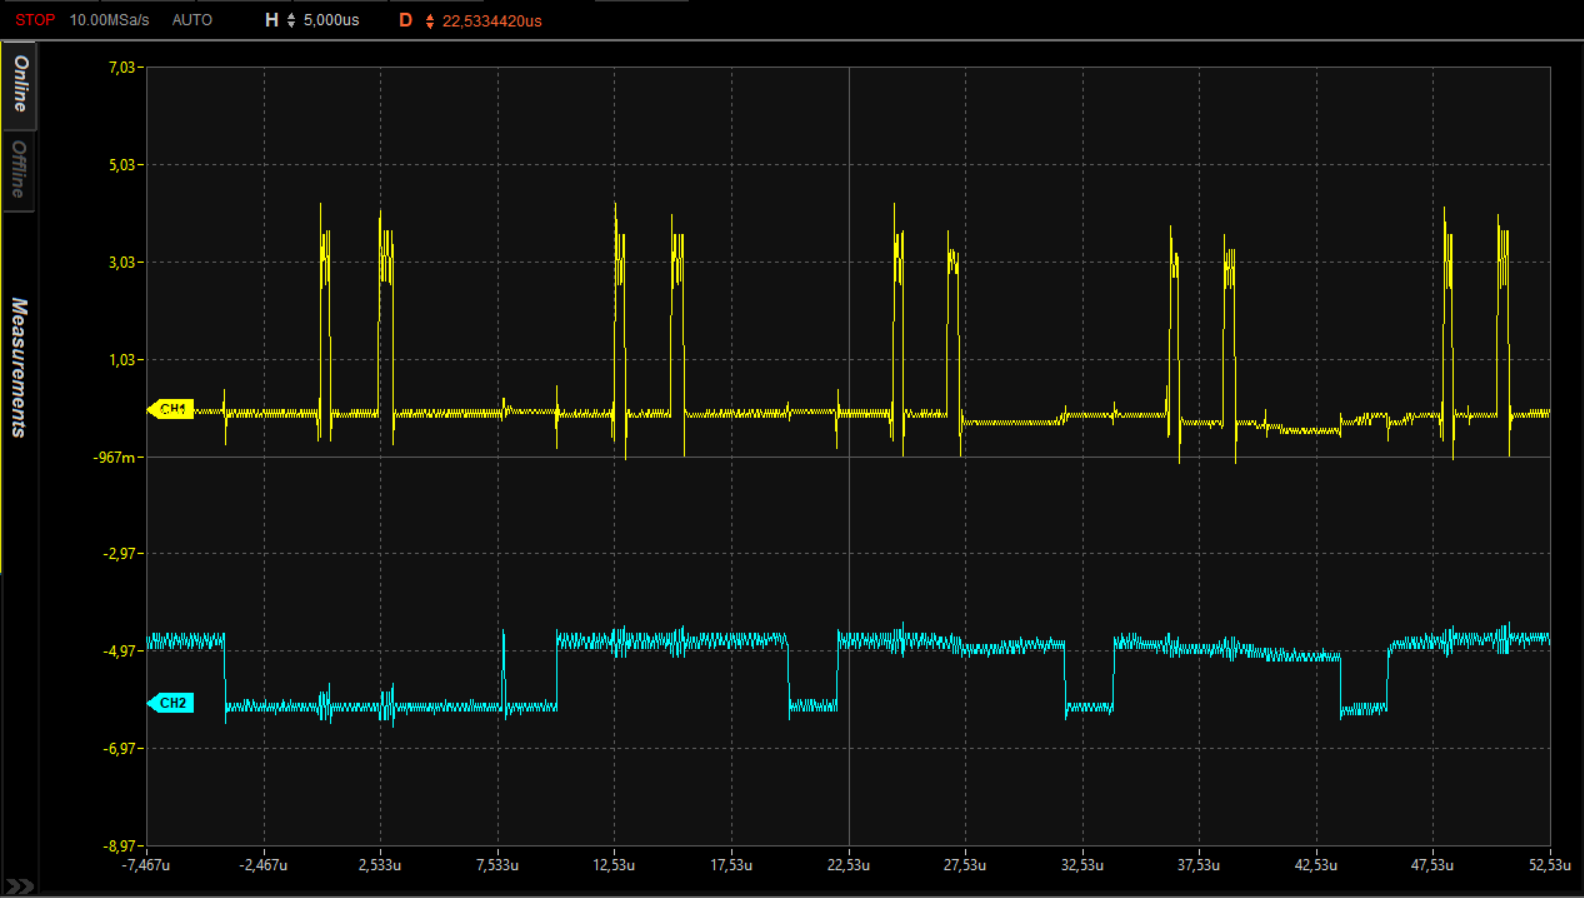
\includegraphics[scale =0.40]{images/spi_write_graph/spi_write_graph3.PNG}
    \caption{Forme d'onda che rappresentano MOSI e CS}
    \label{fig:spi_graph1}
\end{figure}
\newline
Il canale 1 rappresenta il pin MOSI, invece il canale 2 rappresenta il pin CS, si può notare che il CS risulta invertito dopo la prima scrittura. La scrittura inizia quando il CS viene portato a livello alto, infatti si può notare che il MOSI riceve due byte, e dopo averli ricevuti il CS ritorna a livello basso.\newline
\newpage
Sul componente vengono scritti due byte che contengono la configurazione del componente e il dato da scrivere, nel nostro caso i due byte sono 0x3F e 0xFF :
\begin{figure}[h]
    \centering
    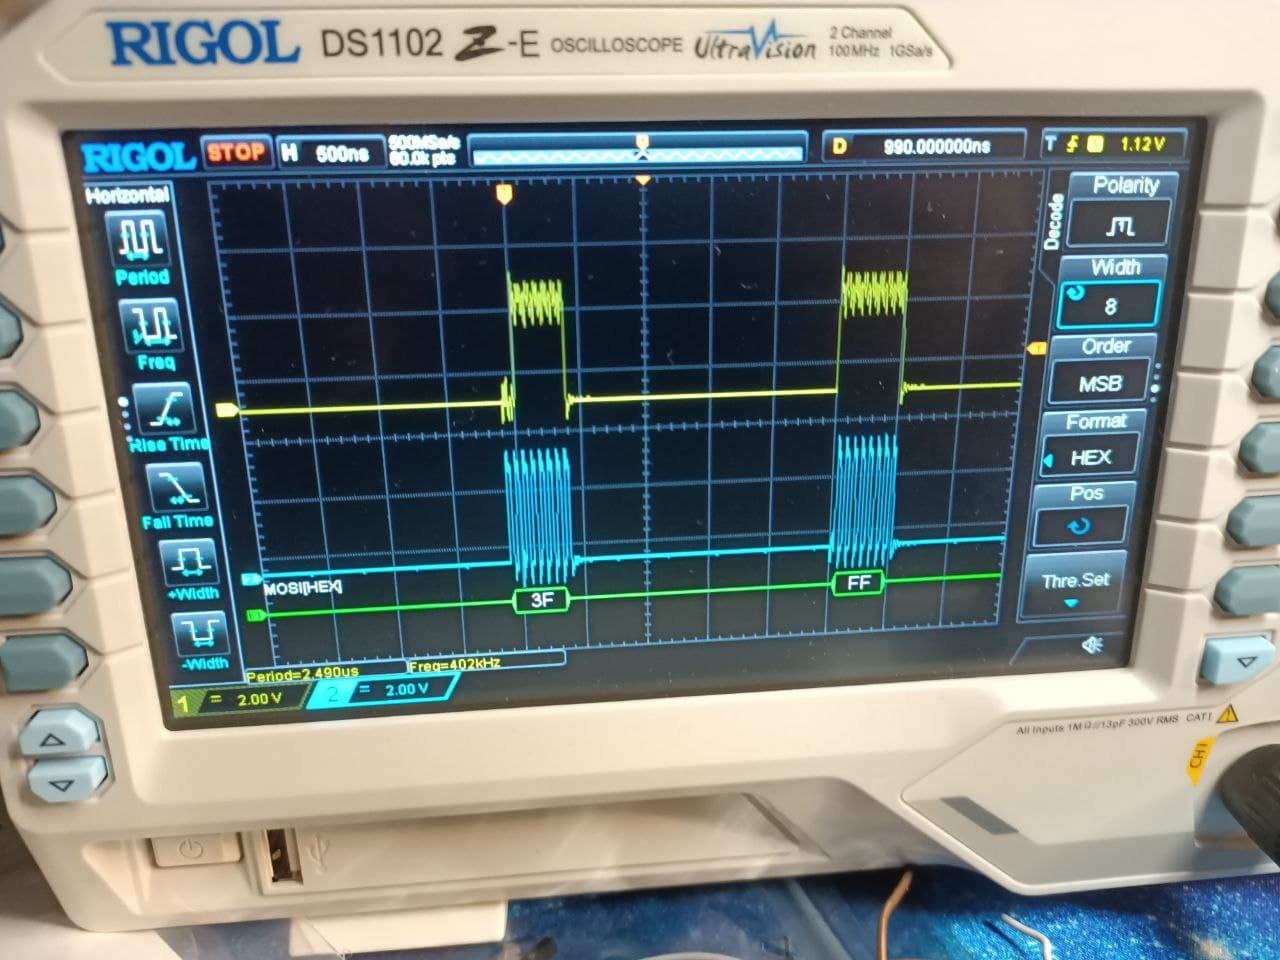
\includegraphics[scale =0.30]{images/spi_write_graph/spi_write_graph4.PNG}
    \caption{Forme d'onda che rappresentano MOSI e SCKL}
    \label{fig:spi_graph2}
\end{figure}
\newpage
A questo punto si vuole verificare la tensione del pin $V_{outA}$, utilizzando l'oscilloscopio, per verificare se questa misura esattamente 0V \newline
\begin{figure}[h]
    \centering
    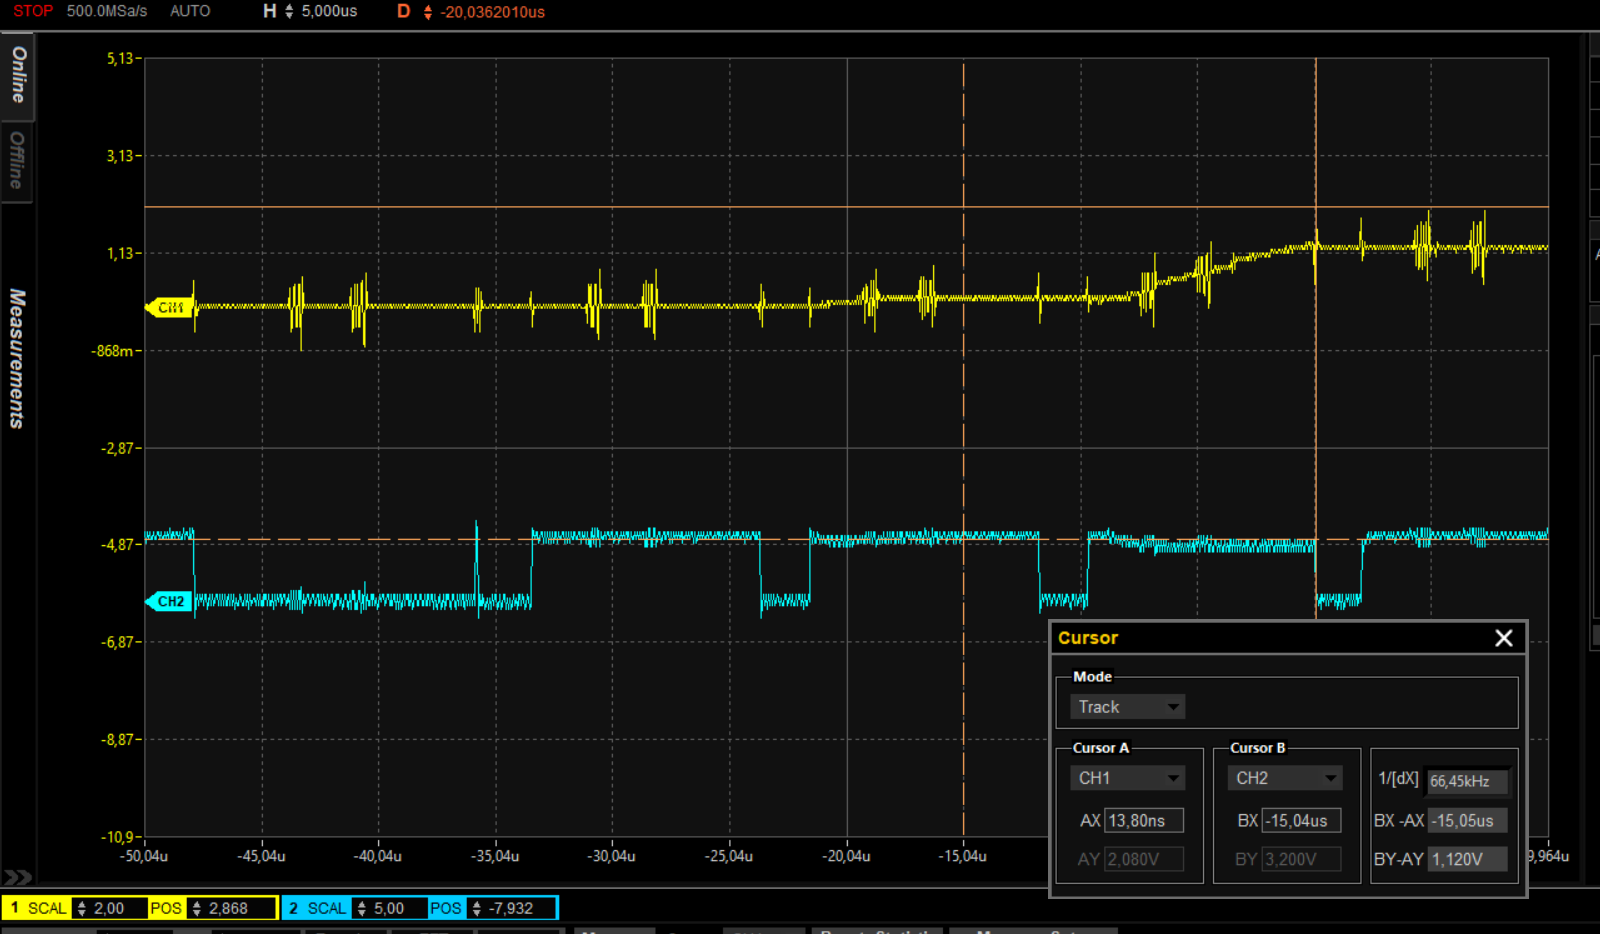
\includegraphics[scale =0.40]{images/spi_write_graph/spi_write_graph5.PNG}
    \caption{Forme d'onda che rappresentano $V_{outA}$ e CS}
    \label{fig:spi_graph2}
\end{figure}
\newline
Come da figura si nota che la tensione del pin $V_{outA}$ aumenta alle ultime due scritture.
e ci si aspetta che La tensione risultante sia 2.048V, ma quando viene misurata è di circa 2.080V in alcuni punti.\newline
E' stato ipotizzato la presenza di un errore nell'API di RTEMS per la gestione del bus SPI, per questo motivo è stata aperta una 'issue' nel repository del'ing. Marques per avere più chiarimenti lato software.\newline
L'ing. Marques ha fato notare che la API di RTEMS non supporta i componenti 'write-only', ma solo i componenti che hanno comunicazione 'full-duplex' dove la Rasbperry Pi per mandare un byte allo 'slave-deviceì deve prima ricevere un byte ('dummy byte'), altrimenti il byte da mandare rimane bloccato sul TX FIFO finché la Raspberry Pi non riceve il 'dummy byte'.\newline
Da questa affermazione si è sicuri che il problema non è la Raspberry Pi, ma risiede nelle API di RTEMS.
\textbf{L'analisi di questo programma è attualmente in corso}.\newline
La verifica di quest'ultimo programma rende chiara l'importanza della validazione e della verifica delle API, prima dello sviluppo di un applicativo più complesso che deve utilizzarle tutte insieme.\newline
%L'ing. Marques ha fatto notare che la API di RTEMS non supporta i componenti 'write-only', ma solo i componenti che hanno una comunicazione 'full-duplex' ed è probabilmente questo il problema.\newline
\textbf{Quindi in conclusione si è riuscito a validare tutte le API prefissate tranne quella della SPI.\newline
}
\chapter{Conclusioni}
Il tirocinio denominato "RTEMS su Raspberry Pi per applicazioni real-time" è stato proposto dalla BIS-Italia, sezione italiana della British Interplanetary Society società storica britannica di cui sono membro. \newline 
Il lavoro consisteva in un primo approccio di RTEMS su Raspberry Pi, e nella creazione di documentazione e applicativi di alcune interfacce (UART, GPIO, SPI, I2C) che potrebbero essere utili per qualunque utente volesse fare lo stesso percorso.\newline
La documentazione prodotta è la guida per il 'porting' di RTEMS su Raspberry Pi che illustra tutti i passaggi necessari da eseguire.\newline
La guida è il risultato di tanti tentativi di porting falliti, per via dei manuali "datati", e risolti grazie all'aiuto dell'ing. Basile. Per questo motivo l'attività di 'porting' ha portato più tempo del previsto, ed è il requisito base per procedere alla creazione degli applicativi poiché viene impostato l'ambiente di sviluppo.\newline
Lo scopo della creazione degli applicativi, oltre a fornire degli applicativi utili per comprendere se i componenti in possesso non presentano guasti, è anche quello di validare le API di RTEMS e quindi verificare il loro funzionamento. Essendo un progetto 'open-source', è probabile che alcune funzionalità non siano state implementate completamente e in modo corretto, per questo motivo viene fatta la validazione per capire se mancano delle API essenziali per un futuro progetto. All'inizio di questa attività ho avuto la possibilità di fare un incontro con l'ing. Lastri , che ha già lavorato su RTEMS, e mi ha dato una spiegazione generale di RTEMS con esempi di applicativi base.\newline
Lo sviluppo ha occupato molto tempo soprattutto per i programmi di validazione delle interfacce I2C e SPI, poiché si pensava che fossero presenti delle API di RTEMS che potessero gestirle, e quindi non era prevista la creazione dei driver da associare ai componenti.\newline
La validazione oltre allo sviluppo ha bisogno di dati o grafici che possano provare l'effettivo funzionamento dell'applicativo, per questo motivo mi sono munito di un oscilloscopio per verificare che i segnali vengano mandati come previsto. Prima di utilizzare questo strumento ho dovuto consultare dei manuali, poiché è la prima volta che lo utilizzo. L'oscilloscopio è stato molto utile per verificare i tempi di risposta dell'applicativo, caratteristica molto importante nei software real-time che determina anche il risultato di una computazione.\newline
Durante questo tirocinio ho potuto affrontare gli aspetti software, dalla creazione di un semplice programma "hello world" alla creazione di driver per dei componenti aggiuntivi da integrare, e gli aspetti hardware, dalla lettura dei datasheet alla saldatura dei componenti, di un applicativo real-time.\newline
Nonostante il lavoro sia stato fatto totalmente in modalità 'smart-working' ho potuto avere molto supporto dalla BIS-Italia per ogni eventuale dubbio.\newline
Questo lavoro può essere utilizzato come punto di partenza per lo sviluppo di applicativi RTEMS su Raspberry Pi, oppure per validare le API in diverse casistiche, magari anche 'mission-critical'.\newline
Inoltre BIS-Italia prevede di utilizzare RTEMS su Raspberry Pi per il progetto di una replica in scala 1:3 di ExoMars Rover che verrà utilizzato per divulgazione.\newline
Il tirocinio è stato svolto con l'aiuto dei membri di BIS-Italia e la collaborazione di Microchip, e mi posso ritenere soddisfatto dell'esperienza sia a livello di competenze che a livello personale.\newline

\printbibliography

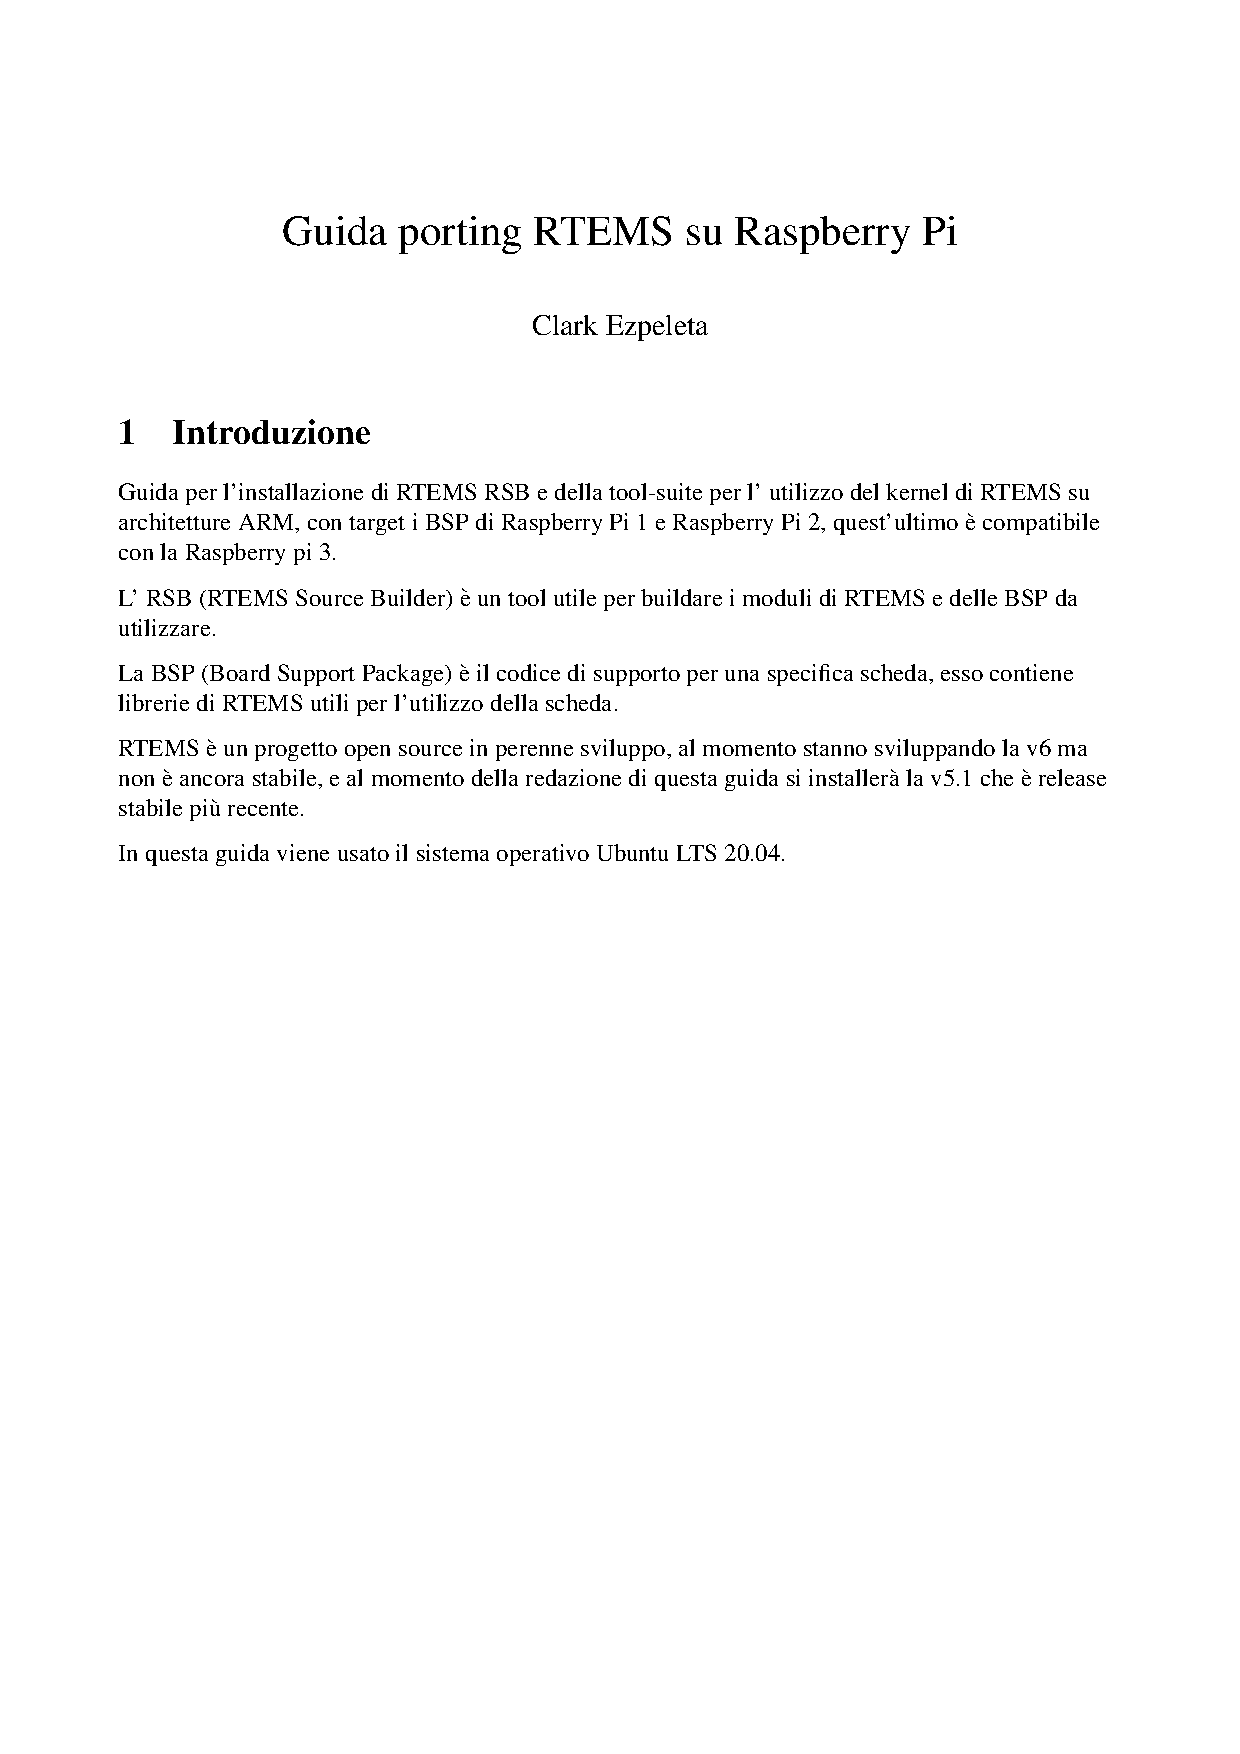
\includepdf[pages={-}]{Guida_porting_RTEMS.pdf}

\chapter*{Ringraziamenti}

E' doveroso dire che questo percorso durato tre anni, non sarebbe stato possibile farlo da solo, ma grazie a tutte le persone che ho incontrato e mi sono rimaste accanto in questi anni sono riuscito a concluderlo, e per questo motivo voglio dedicare queste ultime pagine a voi.\newline


Innanzitutto devo dire grazie alla mia famiglia che mi ha sempre sostenuto in qualunque scelta io abbia fatto, e senza il loro supporto non sarei riuscito a raggiungere questo traguardo. Grazie di cuore per tutto, vi voglio bene.\newline


Vorrei ringraziare il mio relatore, il prof. Sorrenti, e il mio tutor aziendale, il prof.Braione, che hanno creduto in questo tirocinio e nonostante i piccoli ostacoli burocratici sono riusciti darmi la possibilità di svolgerlo.\newline


Ovviamente devo ringraziare tantissimo colui che ha progettato il tirocinio, ovvero l'ing. Bernardini, che mi ha seguito e guidato durante tutto il percorso ed è sempre stato molto disponibile nonostante i suoi mille impegni. Grazie per la fiducia che mi hai dato nell'assegnarmi questo progetto.\newline


Devo ringraziare l'ing.Kubler di Microchip Technologies che mi ha gentilmente offerto i componenti aggiuntivi, ed è stato molto disponibile a dare supporto tecnico.\newline


Grazie alla BIS-Italia, e quindi anche alla British Interplanetary Society, di cui sono fiero di essere membro, non solo perché é la più antica associazione di astronautica al mondo, ma anche perché è un associazione che offre opportunità uniche per crescere professionalmente.\\
Mi sono associato due anni e mezzo fa eppure ho potuto partecipare a molti seminari e attività, tra cui quella che mi ha fatto veramente sentire parte del gruppo ovvero il Focus Live Milano 2019.\newline

Tra i membri della BIS devo ringraziare ing. Bernardini, ing. Basile, ing. Viglianti, ing. Kubler, un team di ingegneri che mi hanno dato una mano preziosa e che senza sarei rimasto bloccato al primo step.\newline

Ringrazio l'ing. Lastri e l'ing. Marques par la disponibilità e l'aiuto che mi hanno dato in alcune fasi del tirocinio.\newline

Voglio ringraziare zia Bruna, che ha sempre fatto il tifo per me e mi ha costantemente spronato a dare il massimo. Grazie mille di tutti i preziosi consigli che mi hanno aiutato quando ne avevo bisogno.\newline

Non posso dimenticare di ringraziare anche i miei compagni di studio. \\
Ai miei colleghi e amici dell'auletta U1, grazie della compagnia e dell'aiuto che mi avete dato in questi anni. \\
Ai miei amici dell'U3 che sono grato di aver conosciuto, grazie per avermi "inglobato" e per aver movimentato molte delle mie giornate, con i concertini e balli improvvisati tra un problema di fisica a un altro.\newline

Ai miei migliori amici Valentina e Jason che nonostante tutto sono sempre stati presenti, soprattutto durante i periodi stressanti delle sessioni d'esame. \newline

Grazie di cuore a tutti!
%E per ultimo ma non meno importante voglio ringraziare anche me stesso, che nonostante le difficoltà e i dubbi sei andato avanti con determinazione, e questo è il risultato che ti sei meritato.


\end{document}
